\documentclass{vkr}
\usepackage[english, russian]{babel} % переносы
\usepackage{graphicx} % для вставки картинок
\graphicspath{{images/}} % путь к изображениям
\usepackage[hidelinks]{hyperref}
\usepackage{float} % определяет метод H для рисунка с переносом на следующую страницу, ели не помещается
\usepackage{pdflscape}
\addto{\captionsrussian}{\renewcommand{\refname}{СПИСОК ИСПОЛЬЗОВАННЫХ ИСТОЧНИКОВ}}
\usepackage{xltabular} % для вставки таблиц
\usepackage{makecell}
\renewcommand\theadfont{} % шрифт в /thead
\usepackage{array} % для определения новых типов столбцов таблиц
\newcolumntype{T}{>{\centering\arraybackslash}X} % новый тип столбца T - автоматическая ширина столбца с выравниванием по центру
\newcolumntype{R}{>{\raggedleft\arraybackslash}X} % новый тип столбца R - автоматическая ширина столбца с выравниванием по правому краю
\newcolumntype{C}[1]{>{\centering\let\newline\\\arraybackslash\hspace{0pt}}m{#1}} % новый тип столбца C - фиксированная ширина столбца с выравниванием по центру
\newcolumntype{r}[1]{>{\raggedleft\arraybackslash}p{#1}} % новый тип столбца r - фиксированная ширина столбца с выравниванием по правому краю
\newcommand{\centrow}{\centering\arraybackslash} % командой \centrow можно центрировать одну ячейку (заголовок) в столбце типа X или p, оставив в оcтальных ячейках другой тип выравнивания
\newcommand{\finishhead}{\endhead\hline\endlastfoot}
\newcommand{\continuecaption}[1]{\captionsetup{labelformat=empty} \caption[]{#1}\\ \hline }
\usepackage{etoolbox}
\AtBeginEnvironment{xltabular}{\refstepcounter{tablecnt}} % подсчет таблиц xltabular, обычные таблицы подсчитываются в классе

\usepackage[tableposition=top]{caption} % подпись таблицы вверху
\captionsetup{strut=off}
\setlength{\intextsep}{0pt} % Vertical space above & below [h] floats
\setlength{\textfloatsep}{0pt} % Vertical space below (above) [t] ([b]) floats
\DeclareCaptionLabelFormat{gostfigure}{Рисунок #2} %подпись рисунка
\DeclareCaptionLabelFormat{gosttable}{Таблица #2} %подпись таблицы
\DeclareCaptionLabelSeparator{gost}{~--~} %разделитель в рисунках и таблицах
\captionsetup{labelsep=gost}
\captionsetup[figure]{aboveskip=10pt,belowskip=4mm,justification=centering,labelformat=gostfigure} % настройка подписи рисунка
\captionsetup[table]{font={stretch=1.41},skip=0pt,belowskip=0pt,aboveskip=8.5pt,singlelinecheck=off,labelformat=gosttable} % настройка подписи таблицы

\setlength{\LTpre}{8mm} % отступ сверху таблицы
\setlength{\LTpost}{6mm} % отступ снизу таблицы

\usepackage{enumitem}
\setlist{nolistsep,wide=\parindent,itemindent=*} % отступы вокруг списков, выравнивание с учетом разделителя

\usepackage{color} %% это для отображения цвета в коде
\usepackage{listings} %% листинги кода
\setmonofont[Scale=0.7]{Verdana} % моноширный шрифт для листинга

\definecolor{codegreen}{rgb}{0,0.6,0}
\definecolor{codegray}{rgb}{0.5,0.5,0.5}
\definecolor{codepurple}{rgb}{0.58,0,0.82}

\lstset{ %
language=C,                 % выбор языка для подсветки (здесь это С)
numbers=left,               % где поставить нумерацию строк (слева\справа)
numberstyle=\tiny,           % размер шрифта для номеров строк
stepnumber=1,                   % размер шага между двумя номерами строк
numbersep=5pt,                % как далеко отстоят номера строк от подсвечиваемого кода
commentstyle=\color{codegreen},
keywordstyle=\color{magenta},
numberstyle=\tiny\color{codegray},
stringstyle=\color{codepurple},
basicstyle=\linespread{0.95}\ttfamily,
backgroundcolor=\color{white}, % цвет фона подсветки - используем \usepackage{color}
showspaces=false,            % показывать или нет пробелы специальными отступами
showstringspaces=false,      % показывать или нет пробелы в строках
showtabs=false,             % показывать или нет табуляцию в строках
frame=single,              % рисовать рамку вокруг кода
tabsize=2,                 % размер табуляции по умолчанию равен 2 пробелам
captionpos=t,              % позиция заголовка вверху [t] или внизу [b] 
breaklines=true,           % автоматически переносить строки (да\нет)
breakatwhitespace=false, % переносить строки только если есть пробел
escapeinside={\%*}{*)}   % если нужно добавить комментарии в коде
}

\makeatletter % чтобы допускались русские комментарии в листингах
\lst@InputCatcodes
\def\lst@DefEC{%
 \lst@CCECUse \lst@ProcessLetter
  ^^80^^81^^82^^83^^84^^85^^86^^87^^88^^89^^8a^^8b^^8c^^8d^^8e^^8f%
  ^^90^^91^^92^^93^^94^^95^^96^^97^^98^^99^^9a^^9b^^9c^^9d^^9e^^9f%
  ^^a0^^a1^^a2^^a3^^a4^^a5^^a6^^a7^^a8^^a9^^aa^^ab^^ac^^ad^^ae^^af%
  ^^b0^^b1^^b2^^b3^^b4^^b5^^b6^^b7^^b8^^b9^^ba^^bb^^bc^^bd^^be^^bf%
  ^^c0^^c1^^c2^^c3^^c4^^c5^^c6^^c7^^c8^^c9^^ca^^cb^^cc^^cd^^ce^^cf%
  ^^d0^^d1^^d2^^d3^^d4^^d5^^d6^^d7^^d8^^d9^^da^^db^^dc^^dd^^de^^df%
  ^^e0^^e1^^e2^^e3^^e4^^e5^^e6^^e7^^e8^^e9^^ea^^eb^^ec^^ed^^ee^^ef%
  ^^f0^^f1^^f2^^f3^^f4^^f5^^f6^^f7^^f8^^f9^^fa^^fb^^fc^^fd^^fe^^ff%
  ^^^^20ac^^^^0153^^^^0152%
  % Basic Cyrillic alphabet coverage
  ^^^^0410^^^^0411^^^^0412^^^^0413^^^^0414^^^^0415^^^^0416^^^^0417%
  ^^^^0418^^^^0419^^^^041a^^^^041b^^^^041c^^^^041d^^^^041e^^^^041f%
  ^^^^0420^^^^0421^^^^0422^^^^0423^^^^0424^^^^0425^^^^0426^^^^0427%
  ^^^^0428^^^^0429^^^^042a^^^^042b^^^^042c^^^^042d^^^^042e^^^^042f%
  ^^^^0430^^^^0431^^^^0432^^^^0433^^^^0434^^^^0435^^^^0436^^^^0437%
  ^^^^0438^^^^0439^^^^043a^^^^043b^^^^043c^^^^043d^^^^043e^^^^043f%
  ^^^^0440^^^^0441^^^^0442^^^^0443^^^^0444^^^^0445^^^^0446^^^^0447%
  ^^^^0448^^^^0449^^^^044a^^^^044b^^^^044c^^^^044d^^^^044e^^^^044f%
  ^^^^0401^^^^0451%
  %%%
  ^^00}
\lst@RestoreCatcodes
\makeatother


% Режим шаблона (должен быть включен один из трех)
%\ВКРtrue
\Практикаtrue
%\Курсоваяtrue

\newcommand{\Дисциплина}{<<Проектирование и архитектура программных систем>>} % для курсовой
\newcommand{\КодСпециальности}{09.03.04} % Курсовая
\newcommand{\Специальность}{Программная инженерия} % Курсовая
\newcommand{\Тема}{Разработка web сервиса фриланс-биржи} % ВКР Курсовая
\newcommand{\ТемаВтораяСтрока}{}
\newcommand{\ГдеПроводитсяПрактика}{ООО «МЦОБ. Онлайн-сервисы»} % для практики
\newcommand{\РуководительПрактПредпр}{Куркина А. В.} % для практики
\newcommand{\ДолжнРуководительПрактПредпр}{директор} % для практики
\newcommand{\РуководительПрактУнивер}{Чаплыгин А. А.} % для практики
\newcommand{\ДолжнРуководительПрактУнивер}{к.т.н. доцент} % для практики
\newcommand{\Автор}{А. Е. Алексеев}
\newcommand{\АвторРод}{Алексеева А. Е.}
\newcommand{\АвторПолностьюРод}{Алексеева Андрея Евгеньевича} % для практики
\newcommand{\Шифр}{21-06-0181}
\newcommand{\Курс}{4} % для практики
\newcommand{\Группа}{ПО-11б}
\newcommand{\Руководитель}{А. А. Чаплыгин} % для ВКР и курсовой
\newcommand{\Нормоконтроль}{А. А. Чаплыгин} % для ВКР
\newcommand{\ЗавКаф}{А. В. Малышев} % для ВКР
\newcommand{\ДатаПриказа}{«07» апреля 2025~г.} % для ВКР
\newcommand{\НомерПриказа}{1505-с} % для ВКР
\newcommand{\СрокПредоставления}{«13» июня 2025~г.} % для ВКР, курсового

\begin{document}
\maketitle
\ifПрактика{}\else{
   \newpage
\begin{center}
\large\textbf{Минобрнауки России}

\large\textbf{Юго-Западный государственный университет}
\vskip 1em
\normalsize{Кафедра программной инженерии}
\vskip 1em
\ifВКР{
        \begin{flushright}
        \begin{tabular}{p{.4\textwidth}}
        \centrow УТВЕРЖДАЮ: \\
        \centrow Заведующий кафедрой \\
        \hrulefill \\
        \setarstrut{\footnotesize}
        \centrow\footnotesize{(подпись, инициалы, фамилия)}\\
        \restorearstrut
        «\underline{\hspace{1cm}}»
        \underline{\hspace{3cm}}
        20\underline{\hspace{1cm}} г.\\
        \end{tabular}
        \end{flushright}
        }\fi
\end{center}
\vspace{1em}
  \begin{center}
  \large
\ifВКР{
ЗАДАНИЕ НА ВЫПУСКНУЮ КВАЛИФИКАЦИОННУЮ РАБОТУ
  ПО ПРОГРАММЕ БАКАЛАВРИАТА}
  \else
ЗАДАНИЕ НА КУРСОВУЮ РАБОТУ (ПРОЕКТ)
\fi
\normalsize
  \end{center}
\vspace{1em}
{\parindent0pt
  Студента \АвторРод, шифр\ \Шифр, группа \Группа
  
1. Тема «\Тема\ \ТемаВтораяСтрока»
\ifВКР{
утверждена приказом ректора ЮЗГУ от \ДатаПриказа\ № \НомерПриказа
}\fi.

2. Срок предоставления работы к защите \СрокПредоставления

3. Исходные данные для создания программной системы:

3.1. Перечень решаемых задач:}

\renewcommand\labelenumi{\theenumi)}

\begin{enumerate}
\item проанализировать IT-инфраструктуру подобных сервисов;
\item  разработать концептуальную модель системы управления web сервисом фриланс-биржи на основе подхода к управлению и организации ИТ-услуг ITSM;
\item спроектировать программную систему управления IT-ин\-фра\-струк\-турой сервиса;
\item сконструировать и протестировать программную систему управления IT-инфраструктурой сервиса.
\end{enumerate}

{\parindent0pt
  3.2. Входные данные и требуемые результаты для программы:}

\begin{enumerate}
\item Входными данными для программной системы являются: данные
справочников комплектующих, конфигураций, ПО, критериев качества SLA,
ИТ-услуг; технические данные ИТ-ресурсов; данные входящих заявок на ИТ-ресурсы.
\item Выходными данными для программной системы являются: сформированные заявки на обслуживание ИТ-ресурсов; сформированные запросы на
закупку комплектующих; сведения о выполненных работах по заявкам; статусы заявок; выходные отчеты (инфографика) – по качеству услуг, по состоянию ИТ-ресурсов, по деятельности ИТ-отдела, по стоимости обслуживания
ИТ-ресурсов, воронка заявок.
\end{enumerate}

{\parindent0pt

  4. Содержание работы (по разделам):
  
  4.1. Введение.
  
  4.1. Анализ предметной области.
  
4.2. Техническое задание: основание для разработки, назначение разработки,
требования к программной системе, требования к оформлению документации.

4.3. Технический проект: общие сведения о программной системе, проект
данных программной системы, проектирование архитектуры программной системы, проектирование пользовательского интерфейса программной системы.

4.4. Рабочий проект: спецификация компонентов и классов программной системы, тестирование программной системы, сборка компонентов программной системы.

4.5. Заключение.

4.6. Список использованных источников.

5. Перечень графического материала:

\списокПлакатов

\vskip 2em
\begin{tabular}{p{6.8cm}C{3.8cm}C{4.8cm}}
Руководитель \ifВКР{ВКР}\else работы (проекта) \fi & \lhrulefill{\fill} & \fillcenter\Руководитель\\
\setarstrut{\footnotesize}
& \footnotesize{(подпись, дата)} & \footnotesize{(инициалы, фамилия)}\\
\restorearstrut
Задание принял к исполнению & \lhrulefill{\fill} & \fillcenter\Автор\\
\setarstrut{\footnotesize}
& \footnotesize{(подпись, дата)} & \footnotesize{(инициалы, фамилия)}\\
\restorearstrut
\end{tabular}
}

\renewcommand\labelenumi{\theenumi.}

   \abstract{РЕФЕРАТ}

Объем работы равен \formbytotal{lastpage}{страниц}{е}{ам}{ам}. Работа содержит \formbytotal{figurecnt}{иллюстраци}{ю}{и}{й}, \formbytotal{tablecnt}{таблиц}{у}{ы}{}, \arabic{bibcount} библиографических источников и \formbytotal{числоПлакатов}{лист}{}{а}{ов} графического материала. Количество приложений – 2. Графический материал представлен в приложении А. Фрагменты исходного кода представлены в приложении Б.

Перечень ключевых слов: коммерческий сайт, Система, фриланс, заказчик, услуги, сервисы, исполнитель, автоматизация, информационные технологии, веб-форма,  REST, API, база данных, подсистема, компонент, модуль, сущность, информационный блок, метод, администратор, пользователь, web-сайт.

Объектом разработки является web сервис фриланс биржа, предназначенной для поика заказчиком исполнителей для конкретной задачи и последующей их коммуникации.

Целью выпускной квалификационной работы является разработка сервиса для удобного удалённого взаимодействия заказчика с исполнителем.

В процессе создания сайта были выделены основные сущности путем создания информационных блоков, использованы классы и методы модулей, обеспечивающие работу с сущностями предметной области, а также корректную работу web-сайта.

При разработке сайта использовались такие инструменты, как язык программирования Python, фреймворк для разработки backend части сайта Django, СУБД PostgreSQL.

Разработанный сайт был успешно разработан и протестирован.

\selectlanguage{english}
\abstract{ABSTRACT}
  
The volume of work is \formbytotal{lastpage}{page}{}{s}{s}. The work contains \formbytotal{figurecnt}{illustration}{}{s}{s}, \formbytotal{tablecnt}{table}{}{s}{s}, \arabic{bibcount} bibliographic sources and \formbytotal{числоПлакатов}{sheet}{}{s}{s} of graphic material. The number of applications is 2. The graphic material is presented in annex A. The layout of the site, including the connection of components, is presented in annex B.

List of keywords: commercial site, System, freelance, customer, services, services, performer, automation, information technology, web form, REST, API, database, subsystem, component, module, entity, information block, method, administrator, user, web-site.

The object of development is a web service freelance exchange, designed to find the customer performers for a particular task and their subsequent communication.

The purpose of graduate qualification work is to develop a service for convenient remote interaction between the customer and the performer.

In the process of creating the site were identified the main entities by creating information blocks, used classes and methods of modules that provide work with the entities of the subject area, as well as the correct operation of the web-site.

During the site development such tools as Python programming language, Django framework for developing the backend part of the site, PostgreSQL DBMS were used.

The developed site was successfully developed and tested.

\selectlanguage{russian}
}\fi
\tableofcontents
\section*{ОБОЗНАЧЕНИЯ И СОКРАЩЕНИЯ}

БД -- база данных.

ИС -- информационная система.

ИТ -- информационные технологии. 

ФБ -- фриланс-биржа.

ПО -- программное обеспечение.

РП -- рабочий проект.

СУБД -- система управления базами данных.

ТЗ -- техническое задание.

ТП -- технический проект.

ER (Entity Relationship) -– модель проектирования данных в виде отношений "<сущность–связь">.

UML (Unified Modelling Language) -- язык графического описания для объектного моделирования в области разработки программного обеспечения.

\ifПрактика{}\else{\section*{ВВЕДЕНИЕ}
\addcontentsline{toc}{section}{ВВЕДЕНИЕ}

Фриланс задал направление развития удалённого взаимодействия сотрудников и руководителя. Так же такая идея взаимодействия заказчика и исполнителя оказалась вполне удобной, так как сотрудник может работать из любой точки мира и регламентировать самому своё рабочее время, так как главным при таком взаимодействии является результат. 

Современные заказчики, видя, как развиваются информационные технологии, пытаются использовать такую идею взаимодйствия выгодно для своего бизнеса, поэтому оставляют свои заказы на проекты в сфере информационных технологий на подобных биржах. С их помощью заказчи может за определённую сумму отобрать необходимого кандидата и получить полноценный результат в определённый срок.

Главной задачей профессионально построенного сервиса является превращение посетителя, зашедшего на сайт, в пользователя, который будет активно пользоваться предоставляемыми услугами сайта.

\emph{Цель настоящей работы} – разработка web сервиса фриланс биржи для удобного взаимодействия заказчиков и исполнителей. Для достижения поставленной цели необходимо решить \emph{следующие задачи:}
\begin{itemize}
\item провести анализ предметной области;
\item разработать концептуальную модель web-сайта;
\item спроектировать web-сайт;
\item реализовать сайт средствами web-технологий.
\end{itemize}

\emph{Структура и объем работы.} Отчет состоит из введения, 4 разделов основной части, заключения, списка использованных источников, 2 приложений. Текст выпускной квалификационной работы равен \formbytotal{lastpage}{страниц}{е}{ам}{ам}.

\emph{Во введении} сформулирована цель работы, поставлены задачи разработки, описана структура работы, приведено краткое содержание каждого из разделов.

\emph{В первом разделе} на стадии описания технической характеристики предметной области приводится сбор информации о подобных уже существующих сервисах, которые предоставляют услуги фриланса.

\emph{Во втором разделе} на стадии технического задания приводятся требования к разрабатываемому сервису.

\emph{В третьем разделе} на стадии технического проектирования представлены проектные решения для web-сайта.

\emph{В четвертом разделе} приводится список классов и их методов, использованных при разработке сайта, производится тестирование разработанного сайта.

В заключении излагаются основные результаты работы, полученные в ходе разработки.

В приложении А представлен графический материал.
В приложении Б представлены фрагменты исходного кода. 
}\fi
\section{Анализ предметной области}
\subsection{Фриланс биржи. История возникновения фриланса}

Термин фриланс (от англ. freelance) возник от слова фрилансер, что в переводе с английского переводится как внештатный сотрудник. Ввод данного термина приписывают британскому поэту и историку Вальтеру Скотту -- он его использовал ещё в романе "Айвенго" 1819 года выхода, где дословно переводя с английского термин обозначается "вольный копейщик".

Но точный период зарождения такого понятия, как фриланс, назвать сложно, но точно можно сказать, что в 90-х годах появлялись первые удалённые работники. Выделить можно один из первых сервисов Guru.com, основанный в 1998 году. Позже, в 1999 году, появилась биржа ELance.

В 2000-х годах, в виду массового развития высокоскоростного интернета, произошёл бум фриланс-бирж. Так же данному явлению способствовали появление удобных платёжных систем и рост аутсорсинга - западные компании нанимали дешёвых специалистов из менее развитых стран. Яркими представителями этого периода можно считать такие биржи, как oDesk, Freelancer.com и Fiverr. Ещё можно выделить, что в этот период началась активная борьба с мошенниками - внедрение безопасных платежей и системы отзывов.

В 2010-х годах уже обособились гиганты рынка - крупные биржи закрекомендовались основными, появлялись локальные биржи в различных странах. Но так же чем интересен данный период - это появление узкоспециализированных бирж по причине перегрузки крупных платформ. 

\subsection{Как устроены фриланс биржи}

Фриланс-биржи — это сложные цифровые платформы, соединяющие заказчиков и исполнителей через продуманную систему взаимодействий. В их основе лежит четкое разделение сущностей: пользователи (заказчики, фрилансеры, модераторы), проекты с описанием задач, заявки от исполнителей, портфолио работ и финансовые транзакции. Каждый элемент системы обладает своими атрибутами и связями — например, проект включает бюджет, сроки и статус, а заявка содержит ценовое предложение и комментарий фрилансера. Ключевые бизнес-процессы построены вокруг публикации заказов, подачи откликов, безопасных платежей через Escrow-системы и механизмов обратной связи, формирующих репутацию участников.

С технической точки зрения фриланс-биржи используют клиент-серверную архитектуру, где фронтенд (веб и мобильные приложения) взаимодействует с бэкендом через API. Серверная часть включает базы данных для хранения информации, платежные шлюзы для обработки транзакций и сервисы уведомлений. В сложных системах применяется микросервисный подход, разделяющий функционал на модули: аутентификацию, управление проектами, поиск и платежи. Особое внимание уделяется безопасности — шифрование данных (HTTPS, JWT), верификация пользователей и механизмы арбитража для разрешения споров. Для борьбы с мошенничеством внедряются репутационные системы, анализ поведения и модерация контента.

Современные платформы активно используют анализ данных и машинное обучение. Рекомендательные системы предлагают заказчикам подходящих фрилансеров на основе истории заказов и навыков, а исполнителям — релевантные проекты. Алгоритмы выявляют подозрительную активность, например фейковые заказы или попытки обмана при оплате. Отдельное направление — оптимизация ценообразования, где ИИ анализирует рыночные тенденции и подсказывает исполнителям конкурентные ставки. В будущем эти технологии будут развиваться в сторону персонификации, автоматизации рутинных задач (например, составления ТЗ) и интеграции с Web3 — децентрализованными биржами на блокчейне.

\subsection{Пример фриланс биржи}

Как пример фриланс биржи можно взять такой веб-сервис, как FL.ru (ранее Free-lance.ru). Он является одной из старейших фриланс бирж, которая актуальна до сих пор, так как в отличии от Kwork с его фиксированными услугами, FL сохраняет свою стандартную модель взаимодействия заказчика и исполнителя в формате аукционов. 

Ключевыми особенностями данного сервиса являются аукционная система и безопасность сделок. 

Аукционную систему можно представить в виде данной схемы: заказчик публикует техническое задание, а исполнители подают свои заявки с ценовыми предложениями. Для заказчика это выгодно, так как он может получить выполнение необходимой задачи за как можно меньшую цену, но для исполнителей это может обернуться тем, что новички намеренно будут занижать цену ради первых отзывов. В данном случае у опытных специалистов открывается несколько путей: либо занижать ещё сильнее цену, либо искать другую задачу.

Безопасность сделок на данном сервисе заключается в том, что средства замораживаются до подтверждения выполнения работы. При данной системе положительные стороны есть как для заказчика, так как если работа не была выполнена - он может вернуть средства, так и для исполнителя, так как все транзакции проходят через сам сервис.

Так же при анализе сервиса FL.ru были выявлены и слабые стороны.

Первой слабой стороной можно назвать высокую комиссию - здесь она составляет 20\% с каждой сделки для обычных пользователей и 10\% для пользователей подписки PRO.

Второй стороной является то, что на данном сервисе отсутствует чёткий стандарт написания ТЗ, в связи с чем могут возникать различные споры и конфликты между заказчиком и исполнителем.
\section{Техническое задание}
\subsection{Основание для разработки}

Основанием для разработки является задание на выпускную квалификационную работу бакалавра "<Разработка web сервиса фриланс-биржи">.

\subsection{Цель и назначение разработки}

Основной задачей выпускной квалификационной работы является разработка web-сервиса, реализующего возможности фриланс биржи.

Посредством разработки web-сервиса планируется реализовать возможности фриланс-биржи. Исходя из этого, основную цель предлагается рассмотреть в разрезе двух групп подцелей.

Задачами данной разработки являются:
\begin{itemize}
\item создание сущностей исполнителя и заказчика;
\item реализация функций взаимодействия между данными сущностями;
\item реализация формы просмотра задачи;
\item реализация системы удержания средств до выполнения задания;
\item реализация графического отображения функций сайта для взаимодействия с пользователем.
\end{itemize}

\subsection{Описание проекта "<FreelanceDay!">}

Данный сервис представляет собой систему взаимодействия между двумя типами пользователей -- заказчик и исполнитель. Взаимодействие обоих типов пользователей происходит вокруг задач. Так же, на равне с задачами, пользователи имеют дело с платёжной системой, которая является прикреплённым вознаграждением за задачи. Взаимодействие пользователя с самим сервисом происходит на основе клиент-серверной архитектуры.

Сервис можно разделить на 3 взаимодействующие между собой подсистемы: администрирование (administration), система задач (task system) и платёжная система (payment system).

\subsubsection{Подсистема "<Администрирование">. Сущности исполнителя и заказчика}

Подсистема "<Администрование"> отвечает за хранение информации о пользователях, определение их роли а так же за авторизацию на сайте. Всего в сервисе существует 2 типа пользователя -- заказчик и исполнитель. У каждой из сущностей есть свой набор полей, который частично отличается. 

Сущность заказчика -- это "поставщик" задач. Он может выкладывать на сервис задачи, выбирать кандидатов из списка откликнувшихся и завершать задачу. После полного выполнения заказчик может оставить оценку на исполнителя.

Сущность исполнителя -- это "охотник" на задачи. Он выбирает из списка готовых на сервисе задач, оставляет отклик и берётся за выполнение задачи. После выполнения задачи исполнитель получает очки опыта, которые позволяют повысить уровень, который помогает получать более сложные и высокооплачиваемые задачи.

\subsubsection{Подсистема "<Система задач">. Сущность задачи}

Подсистема "<Система задач"> представляет собой воплощение сущности "<Задача">. Напрямую с данной подсистемой взаимодействуют сущности заказчика и исполнителя.

Сущность задачи -- это объект, который создаётся заказчиком на сервисе с помощью специальных инструментов, представленных сайтом. Заказчик описывает данный объект такими основными признаками, как название задачи, её описание, стоимость и сложность выполнения задачи. После создания она находится в списке доступных для отклика задач и спустя время она обрастает таковыми. Когда исполнитель выбран -- объект находится в статусе, который условно можно назвать "<На выполнении">. Если исполнитель выполнил задачу - он переводит задачу в статус "<На завершении">, а заказчик в свою очередь переводит задачу в статус "<Завершено">, после чего происходит взаимодействие с подсистемой "<Платёжная система"> для перевода средств на виртуальный счёт исполнителя.

\subsubsection{Подсистема "<Платёжная система">. Сущности виртуального счёта и платежа}

Подсистема "<Платёжная система"> представляет собой воплощение сущностей "<Виртуальный счёт"> и "<Платёж"> и предназначена для управления денежными средствами, которые находятся внутри сервиса. 

Сущность виртуального счёта -- это объект, который является вместилещем для денежных средств кадого пользователя и задачи. В зависимости от роли у счёта могут меняться права, например: для роли заказчика счёт доступен только на внесение средств и исходящий перевод, для роли исполнителя наоборот -- только на вывод и входящий перевод, а для счёта сущности задачи доступен на входящие и исходящие переводы.

Сущность платежа -- это объект, который можно назвать "<перевозчиком"> платежей. Т. е. он забирает денежные средства из одной точки (первый виртуальный счёт) и привозит их во вторую точку (второй виртуальный счёт). Так же данный объект используется, как хранитель истории операций -- можно просмотреть когда проходил платёж, отравителя, получателя и его сумму.

\subsection{Требования пользователя к web сервису}

Сервис должен включать в себя следующий функционал:
\begin{itemize}
    \item авторизация пользователя;
    \item регистрация на сервисе;
    \item отображение личного кабинета пользователя;
    \item пополнение средств заказчиком;
    \item вывод средств пользователем;
    \item отображение списка доступных задач;
    \item создание задачи заказчиком, зачисление на неё средств;
    \item отображение информации о задаче;
    \item отклик на задачу исполнителями;
    \item выбор исполнителя заказчиком из списка кандидатов;
    \item завершение выполнения задачи со стороны как исполнителя, так и заказчика;
    \item перечисление средств за выполнение задачи на виртуальный счёт исполнителя.
\end{itemize}

На рисунке ~\ref{tz1:image} представлен макет страницы просмотра доступных задач.

\begin{figure}[ht]
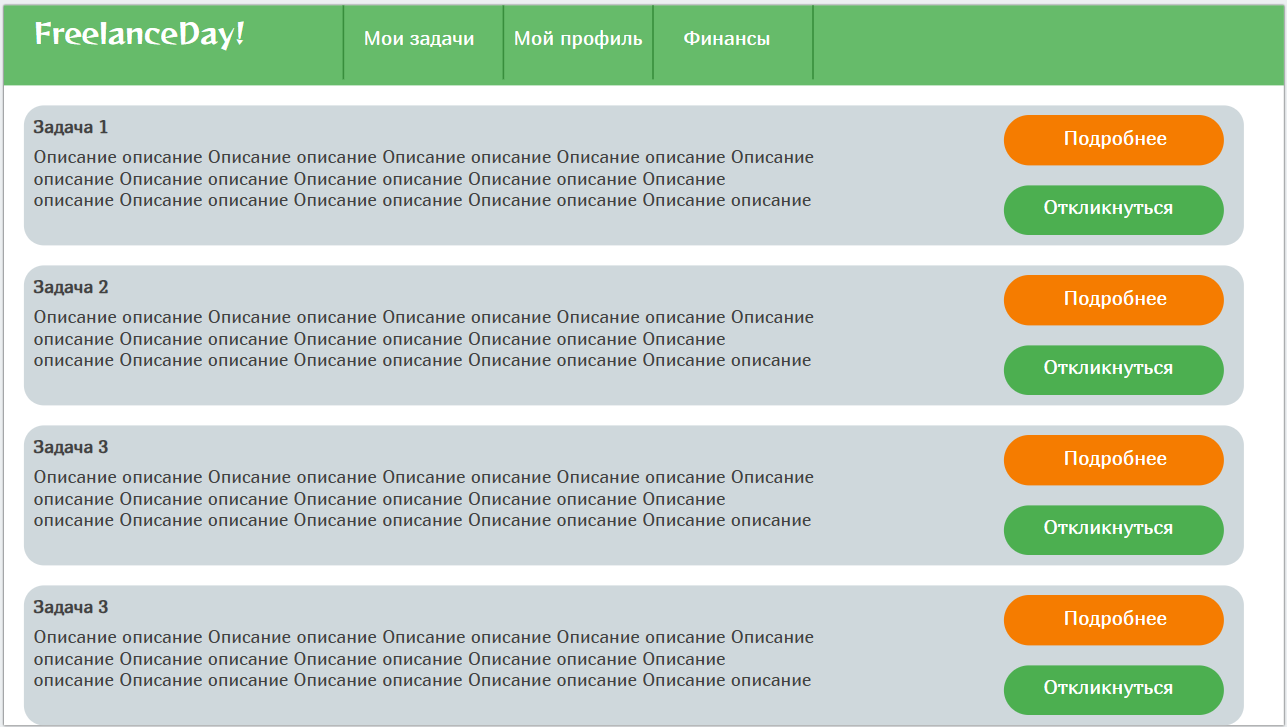
\includegraphics[width=1\linewidth]{tz0s1.png}
\caption{Макет страницы просмотра доступных задач}
\label{tz1:image}
\end{figure}
%\vspace{-\figureaboveskip} % двойной отступ не нужен (можно использовать, если раздел заканчивается картинкой)

Здесь представлены сами задачи, их краткое описание и кнопки для отклика на задачу и для просмотра подробной информации о задаче. Так же на каждой странице можно увидеть кнопки в шапке страницы -- "<Мои задачи">, "<Мой профиль"> и "<Финансы"> -- они переносят пользователя на соответствующую страницу.

На рисунке ~\ref{tz2:image} представлен макет страницы входа на сайт.
\clearpage

\begin{figure}[ht]
	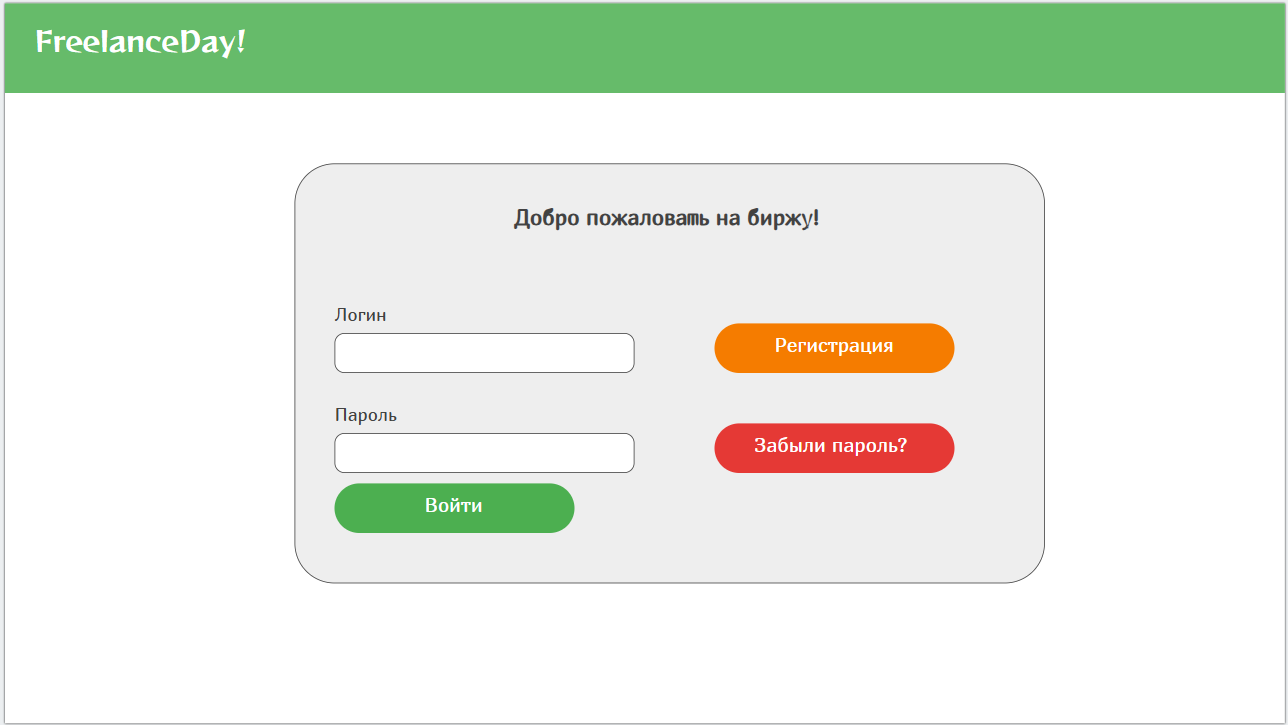
\includegraphics[width=1\linewidth]{tz0s2.png}
	\caption{Макет страницы входа на сайт}
	\label{tz2:image}
\end{figure}

Здесь представлены поля для вввода логина, пароля, кнопки для входа на сайт, перехода на страницу регистрации и для перехода на страницу восстановления пароля.

На рисунке ~\ref{tz3:image} представлен макет страницы просмотра информации о пользователе.
\clearpage

\begin{figure}[ht]
	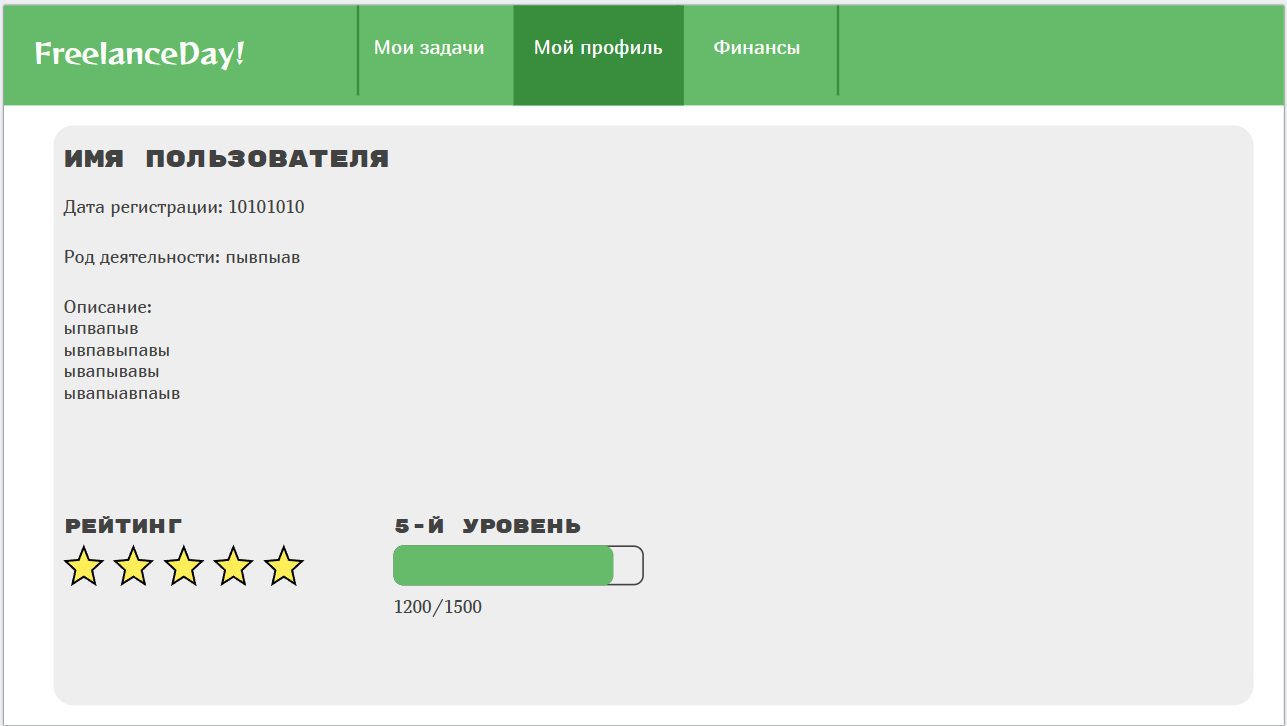
\includegraphics[width=1\linewidth]{tz0s3.png}
	\caption{Макет страницы просмотра информации о пользователе}
	\label{tz3:image}
\end{figure}

Здесь представлены поля, которые отображают доступную информацию о пользователе - его имя, дату регистрации, описание пользователя, рейтинг на сервисе и уровень.

\subsection{Моделирование вариантов использования}

\subsubsection{Диаграмма прецедентов}

Для разрабатываемого сайта была реализована модель, которая обеспечивает наглядное представление вариантов использования сайта.

Она помогает в физической разработке и детальном анализе взаимосвязей объектов. При построении диаграммы вариантов использования применяется унифицированный язык визуального моделирования UML.

Диаграмма вариантов описывает функциональное назначение разрабатываемой системы. То есть это то, что система будет непосредственно делать в процессе своего функционирования. Она является исходным концептуальным представлением системы в процессе ее проектирования и разработки. Проектируемая система представляется в виде ряда прецедентов, предоставляемых системой актерам или сущностям, которые взаимодействуют с системой. Актером или действующим лицом является сущность, взаимодействующая с системой извне (например, человек, техническое устройство). Прецедент служит для описания набора действий, которые система предоставляет актеру.

На основании анализа предметной области в программе должны быть реализованы следующие прецеденты:
\begin{itemize}
\item авторизация пользователя, определение роли;
\item пополнение виртуального счёта заказчика;
\item создание задачи и перечисление на неё средств;
\item выбор исполнителя;
\item завершение задачи;
\item просмотр списка доступных задач;
\item просмотр подробной информации о задаче;
\item отклик на задачу;
\item отправка задачи на завершение;
\item вывод средств с виртуального счёта исполнителя;
\item выход из аккаунта.
\end{itemize}
\clearpage

\begin{figure}[ht]
	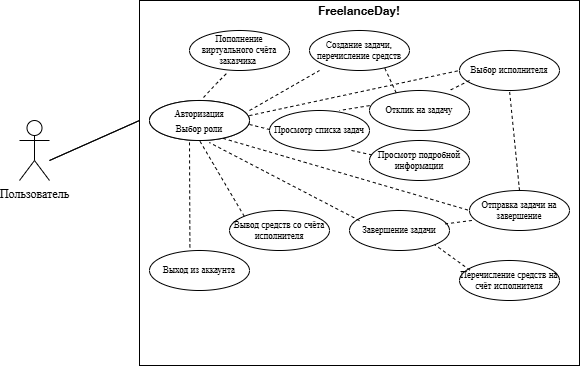
\includegraphics[width=1\linewidth]{useCase.png}
	\caption{Диаграмма прецедентов}
	\label{ucUML:image}
\end{figure}

\subsubsection{Сценарии прецедентов программы}

\begin{enumerate}
\item Сценарий для прецедента "<Авторизация пользователя, определение роли">:
	\begin{itemize}
		\item основной исполнитель: пользователь;
		\item заинтересованные лица и их требования: пользователю необходимо произвести вход на сайт;
		\item предусловие: перед началом работы у пользователя открыта страница входа на сайт;
		\item основной успешный сценарий: пользователь заполняет поля "<Логин"> и "<Пароль"> валидными значениями, нажимает кнопку "<Войти">. Отображается главная страница сайта, материал на странице представлен в зависимости от роли пользователя.
	\end{itemize}
\item Сценарий для прецедента "<Пополнение виртуального счёта заказчика">:
	\begin{itemize}
		\item основной исполнитель: пользователь с ролью "<Заказчик">;
		\item заинтересованные лица и их требования: пользователю необходимо пополнить свой виртуальный счёт;
		\item предусловие: пользователь авторизован на сайте, открыта страница пополнения виртуального счёта;
		\item основной успешный сценарий: пользователь заполняет необходимые поля данными своей карты и поле "<Сумма пополнения"> необходимой суммой, которую хочет получить на свой виртуальный счёт, нажимает кнопку "<Пополнить">, подтверждает свою карту. Отображается информационное сообщение об успешном пополнении, сумма виртуального счёта увеличена на сумму пополнения.
	\end{itemize}
\item Сценарий для прецедента "<Создание задачи и перечисление на неё средств">:
	\begin{itemize}
		\item основной исполнитель: пользователь с ролью "<Заказчик">;
		\item заинтересованные лица и их требования: пользователю необходимо создать задачу;
		\item предусловие: пользователь авторизован на сайте, у пользователя пополнен виртуальный счёт, открыта страница создания задачи;
		\item основной успешный сценарий: пользователь заполняет обязательные поля информацией о задаче, поле "<Сумма"> заполняет валидным значением средств, нажимает кнопку "<Создать задачу">. Отображается информационное сообщение "<Задача успешно создана">.
	\end{itemize}
\item Сценарий для прецедента "<Выбор исполнителя">:
	\begin{itemize}
		\item основной исполнитель: пользователь с ролью "<Заказчик">;
		\item заинтересованные лица и их требования: пользователю необходимо выбрать исполнителя на задачу;
		\item предусловие: пользователь авторизован на сайте, задача в статусе "<Создана"> пользователем создана задача, на задачу откликнулось несколько исполнителей, открыта страница просмотра кандидатов по задаче;
		\item основной успешный сценарий: пользователь просматривает информацию о кандидатах, выбирает исполнителя путём нажатия кнопки "<Выбрать"> в поле соответствующего исполнителя. Отображается информационное сообщение "<Исполнитель успешно выбран"> и информация об выбранном исполнителе.
	\end{itemize}
\item Сценарий для прецедента "<Завершение задачи">:
	\begin{itemize}
		\item основной исполнитель: пользователь с ролью "<Заказчик">;
		\item заинтересованные лица и их требования: пользователю необходимо завершить задачу;
		\item предусловие: пользователь авторизован на сайте, открыта страница с информацией о задаче, на задачу назначен исполнитель и она в статусе "<На завершении">;
		\item основной успешный сценарий: пользователь нажимает кнопку "<Завершить">. Отображается информационное сообщение "<Задача успешно завершена">, задача в статусе "<Завершена">, средства с виртуального счёта задачи перечисляются на виртуальный счёт закреплённого исполнителя.
	\end{itemize}
\item Сценарий для прецедента "<Просмотр списка доступных задач">:
	\begin{itemize}
		\item основной исполнитель: пользователь с ролью "<Исполнитель">;
		\item заинтересованные лица и их требования: пользователю необходимо просмотреть список доступных задач;
		\item предусловие: пользователь авторизован на сайте, открыта страница просмотра списка задач;
		\item основной успешный сценарий: Отображается список доступных задач. У каждой задачи отображаются поля с информацией о задаче и кнопки: "<Подробнее"> и "<Откликнуться">.
	\end{itemize}
\item Сценарий для прецедента "<Просмотр подробной информации о задаче">:
	\begin{itemize}
		\item основной исполнитель: пользователь с ролью "<Исполнитель">;
		\item заинтересованные лица и их требования: пользователю необходимо посмотреть подробную информацию о задаче;
		\item предусловие: пользователь авторизован на сайте, открыта страница просмотра списка задач;
		\item основной успешный сценарий: пользователь нажимает кнопку "<Подробнее"> на необходимой задаче. Отображается страница просмотра полной информации о задаче.
	\end{itemize}
\item Сценарий для прецедента "<Отклик на задачу">:
	\begin{itemize}
		\item основной исполнитель: пользователь с ролью "<Исполнитель">;
		\item заинтересованные лица и их требования: пользователю необходимо откликнуться на выбранную задачу;
		\item предусловие: пользователь авторизован на сайте, открыта страница просмотра задач;
		\item основной успешный сценарий: нажимает кнопку "<Откликнуться"> на выбранной задаче. Кнопка "<Откликнуться"> не отображается, отображается информационное сообщение "<Отклик успешно отправлен!">.
	\end{itemize}
\item Сценарий для прецедента "<Отправка задачи на завершение">:
	\begin{itemize}
		\item основной исполнитель: пользователь с ролью "<Исполнитель">;
		\item заинтересованные лица и их требования: пользователю необходимо задачу, которая находится у него в работе, отправить на завершение;
		\item предусловие: пользователь авторизован на сайте и назначен на задачу, которая находится в статусе "<В работе">, открыта страница просмотра информации о задаче;
		\item основной успешный сценарий: пользователь нажимает кнопку "<Отправить на завершение">. Кнопка "<Отправить на завершение"> не отображается, отображается информационное сообщение "<Задача успешно отправлена на завершение!">, задача в статусе "<На завершении">.
	\end{itemize}
\item Сценарий для прецедента "<Вывод средств с виртуального счёта исполнителя">:
	\begin{itemize}
		\item основной исполнитель: пользователь с ролью "<Исполнитель">;
		\item заинтересованные лица и их требования: пользователю необходимо вывести средства со своего виртуального счёта на банковскую карту;
		\item предусловие: пользователь авторизован на сайте и на его виртуальном счёте присутствуют денежные средства, открыта страница вывода средств;
		\item основной успешный сценарий: пользователь заполняет необходимые поля информацией о банковской карте, поле "<Сумма вывода"> валидным значением, нажимает кнопку "<Вывести">, подтверждает банковскую карту. Отображается информационное сообщение "<Средства успешно отправлены!">, сумма виртуального счёта пользователя уменьшилась на сумму вывода.
	\end{itemize}
\item Сценарий для прецедента "<Выход из аккаунта">:
	\begin{itemize}
		\item основной исполнитель: пользователь;
		\item заинтересованные лица и их требования: пользователю необходимо произвести выход из аккаунта;
		\item предусловие: пользователь авторизован, открыта страница информации о пользователе;
		\item основной успешный сценарий: пользователь нажимает кнопку "<Выйти из аккаунта">. Отображается страница входа на сайт.
	\end{itemize}
\end{enumerate}

\subsection{Требования к оформлению документации}

Разработка программной документации и программного изделия должна производиться согласно ГОСТ 19.102-77 и ГОСТ 34.601-90. Единая система программной документации.

\section{Технический проект}
\subsection{Общая характеристика организации решения задачи}

Необходимо спроектировать и разработать web сервис, который реализует необходимый функционал фриланс-биржи для взаимодействия заказчика и исполнителя.

Web сервис представляет собой набор взаимосвязанных электронных страниц, которые сгруппированы по разделам, содержащие текстовую и графическую информацию. Сайт располагается в Интернете по определенному адресу – доменному имени сайта в виде www.имя\_сайта.ru. Каждая страница web-сайта – это текстовый документ, написанный на языке программирования (HTML, CSS, JavaScript и т.д.).

\subsubsection{Описание используемых технологий и языков программирования}

В процессе разработки проекта используются следующие технологии:

\begin{enumerate}
	\item Backend-часть: язык программирования Python, фреймворк Django, библиотека psycopg2 для взаимодействия с БД, СУБД PostgreSQL.
	\item Frontend-часть: языки программирования TypeScript, HTML, CSS и фреймворк Vue.js.
\end{enumerate}

\subsubsection{Backend-часть сервиса}

Backend-часть любого сервиса -- это, прежде всего, "<мозги"> всего сервиса. Через неё проходит вся логика работы приложения и взаимодействие с необходимыми данными. 

\paragraph{Язык программирования Python}

Python -- это язык прграммирования высокого уровня общего назначения с динамической строгой типизацией и автоматическим управлением памятью. Данный язык программирования достаточно универсален -- он может использоваться для таких задач, как разработка нейросетей, атоматизация тестирования, разработка игр и разработка web-приложений. Достигается такая гибкость благодаря различным библиотекам, которые создаются сообществом неравнодушных к языку пользователей.

\paragraph{Фреймворк Django}

Фреймворк Django -- это фреймворк для создания web-приложений, использующий шаблон проектирования MVC (Model-View-Controller). Состоит сайт на Django из одного или нескольких приложений, которые рекомендуется разрабатывать отчуждаемыми и подключаемыми. Работает фреймворк с множеством различных СУБД (в том числе и PostgreSQL). Из преимуществ так же можно выделить, что у Django присутствует собственный web-сервер, предназначенный для разработки -- он автоматически определяет изменения в файлах исходного кода и при нахождении таковых перезапускается, что в разы ускоряет разработку, но работает web-сервер в однопоточном режиме, потому он и предназначен только для разработки.

Так же можно выделить в данном фреймворке инструмент Django REST Framework, с помощью которого можно создать RESTful API. А API -- это свод определённых правил, по которым клиент общается с сервером, то есть сервер говорит, что он отдаёт необходимую информацию, если ему прислать определённые данные, если же отдать невалидные данные, то сервер их не примет и отдаст ошибку. Посредством API чаще всего происходит "<общение"> frontend-части сайта с его backend-частью, но так же используется для сторонних разработчиков, что бы они могли создавать, например, свои версии моильных приложений web-сервиса или какие-либо полезные скрипты (как пример - "<Вконтакте"> предоставляет подобные инструменты). 

\paragraph{Библиотека psycopg2}

Psycopg2 -- это наиболее популярный адаптер PostgreSQL для Python, в котором реализуется стандарт DB-API 2.0, который заключается в том, что бы у всех библиотек, которые выполняют взаимодействие с базой даннных, был единый интерфейс для работы с ними. Данная библиотека была выбрана не случайно -- она очень хорошо подходит для разработки web-сервиса, ведь она интегрируется с фреймворками создания web-приложений (Django, Flask), позволяя эффективно выполнять CRUD-операции, управлять транзакциями и работать с сложными типами данных. Так же данная библиотека отвечает требованиям безопасности со своим экранированием параметров запроса, что защищает от SQL-инъекций.

\paragraph{СУБД PostgreSQL} 

PostgreSQL -- это свободная объектно-реляционная СУБД. Она, исходя из названия, базируется на языке SQL и помогает в работе с базами данных. Их сильных сторон данной СУБД можно выделить высокопроизводительные механизмы транзакций, расширяемая система встроенных ЯП, возможность индексирования и расширяемость. 

\subsubsection{Frontend-часть сервиса}

Frontend-часть любого сервиса -- это то, с чем уже взаимодействует конечный пользователь. Здесь происходит графическое отображение элементов, необходимых для удобного взаимодействия пользователя с функционалом сервиса. Она являктся этакой прослойкой между пользователем и Backend-частью ("<мозгами">) сайта.

\paragraph{Язык программирования TypeScript}

TypeScript – объектно-ориентированный язык программирования для написания сценариев. По сути, TypeScript является надстройкой над JavaScript, расширяя возможности второго, ведь здесь даже есть возможность скомпилироваться обратно в JavaScript. А отличается он тем, что здесь есть возможность явного статического назначения типов, использования полноценных классов и подключения модулей. Используется TypeScript обычно для написания сценариев работы с web-страницами, отображаемыми web-браузером. Web-бра\-у\-зер интерпретирует код сценария языка TypeScript, и на основе описанных в сценарии действий производит манипуляции с разметкой web-страницы. Посредством языка TypeScript реализуется возможность программирования на стороне клиента. 

\paragraph{Языки разметки HTML и CSS}

HTML (HyperText Markup Language) -- это язык гипертекстовой разметки документов, предназначенный для просмотра web-страниц при помощи браузера. Код таких документов браузером интерпретируются в интерфейс, который отображается на экране монитора. Состоит данный документ обычно из тегов - сначала идёт тег head в котором обычно определяются настройки документа, а после идёт тег body, в котором и заключается вся отображаемая информация. 

CSS (Cascading Style Sheets) -- это язык декорирования и описания внешнего вида документов (обычно используется для HTML-документов). Состоит данный файл из селекторов, в которых перечисляются их свойства и заданные для них значения. В большинстве ситуаций HTML и CSS идут неразрывно рука об руку -- с помощью CSS задаётся внешний вид элементов, указанных в HTML-документе.

\paragraph{Фреймворк Vue.js}

Vue.js -- это opensource JS-фреймворк, предназначенный для создания пользовательских интерфейсов. Из явных преимуществ можно выделить, что его не сложно освоить и легко интегрировать в проекты с использованием других JS-библиотек. Используется здесь компонентный подход, что позволяет разбивать интерфейс на переиспользуемые блоки, а его свойство реактивности автоматически обновляет DOM при изменении данных. Достигаются все преимущества с помощью встроенных инструментов: VueRouter для маршрутизации, Vuex для управления состоянием и CompositionAPI для лучшей организации кода.

\subsection{Компоненты программной системы}

Диаграмма компонентов описывает особенности физического представления разрабатываемой системы. Она позволяет определить архитектуру системы, установив зависимости между программными компонентами, в роли которых может выступать как исходный, так и исполняемый код. Основными графическими элементами диаграммы компонентов являются компоненты, интерфейсы, а также зависимости между ними. На рисунке \ref{comp:image} изображена диаграмма компонентов для проектируемой системы.

\begin{figure}[ht]
	\center{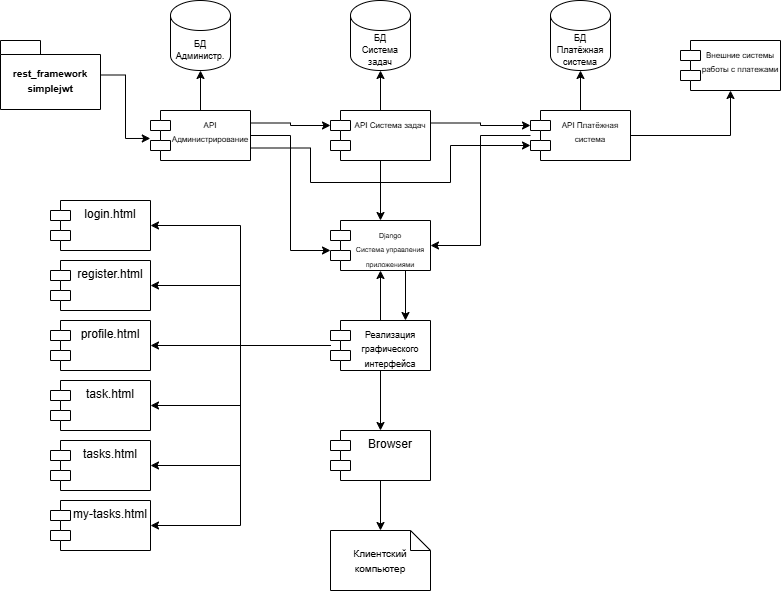
\includegraphics[width=1\linewidth]{components.png}}
	\caption{Диаграмма компонентов}
	\label{comp:image}
\end{figure}

Компненты БД являются базами данных, которые созданы отдельно для каждой подсистемы.

Компонент "<API Администрирование"> отвечает за работу с сущностями пользователей и их авторизацию. Для реализации авторизации используется библиотека simplejwt из пакета rest\_framework. Взаимодействие предусмотрено с подсистемами "<Система задач"> и "<Платёжная система">.

Компонент "<API Система задач"> отвечает за работу с сущностями задач.  Взаимодействие предусмотрено с подсистемами "<Администрирование"> для проверки авторизации в взаимодействия с польхователями и "<Платёжная система"> для получения на задачу средств и дальнейшем переводе их на виртуальный счёт исполнителя.

Компонент "<API Платёжная система"> отвечает за работу с сущностями платежей и платёжных транзакция. Взаимодействие предусмотрено с подсистемами "<Система задач"> для платежей, связанных с задачами, "<Администрирование"> для платежей, связанных с пользователями и внешними системами работы с платежами для пополнения виртуального счёта и вывода средств с него.

Компонент "<Django Система управления приложениями"> является связующим звеном между графическим интерфейсом и API взаимодействующих с ним подсистем. Через него идёт запуск сервера и вызов методов для размещения или получения информации.

Компонент "<Реализация графического интерфейса"> отвечает за отправку отображения графического интерфейса клиенту посредством отправки HTML-документа, который уже расшифровывает компонент "<Browser">. Данные, которые отображаются в HTML-документе, подтягиваются с backend-части при взаимодействии с компонентом "<Django Система управления приложениями"> через отправку запросов к API необходимой подсистемы. 

\subsection{Проект данных программной системы}

Исходя из требований технического задания, программно информационная система должна взаимодействовать с тремя базами данных. Для разработки сервиса требуется использовать СУБД PostgreSQL.

Во-первых, данная СУБД предоставляет надёжную и отказоустойчивую систему хранения данных, что очень важно для платформы, работающей с транзакциями и персональными данными пользователей.

Во-вторых, PostgreSQL показывает свою производительность путём эффективной работы с индексами, что в разы ускоряет поиск задач. Встроенный планировщик запросов оптимизирует выполнение сложных запросов, таких как выборка задач с учетом множества условий.

Третье её преимущество - лёгкая масштабируемость вместе с ростом сервиса. Поддержка табличных пространств позволяет распределять нагрузку по дискам, а механизмы секционирования помогают управлять большими таблицами.

\subsubsection{Описание сущностей клиентской части}

В состав сущностей "<Авторизационные данные">, "<Заказчик">, "<Исполнитель">, "<Задача">, "<Статус задачи">, "<Отклик на задачу">, "<Виртуальный счёт"> и "<История операций">, можно включить атрибуты, представленные в таблицах \ref{login:table} -- \ref{payment:table} соответственно.

\begin{xltabular}{\textwidth}{|l|l|p{1.7cm}|X|}
	\caption{Атрибуты сущности "<Авторизационные данные">\label{login:table}}\\ \hline
	\centrow Поле & \centrow Тип & \centrow Обяза\-тельное & \centrow Описание \\ \hline
	\thead{1} & \thead{2} & \centrow 3 & \centrow 4 \\ \hline
	\endfirsthead
	\continuecaption{Продолжение таблицы \ref{login:table}}
	\thead{1} & \thead{2} & \centrow 3 & \centrow 4 \\ \hline
	\finishhead
	user\_id & integer & + & Уникальный идентификатор пользователя \\ \hline 
	login & character varying & + & Логин пользователя \\ \hline 
	password & character varying & + & Пароль пользователя \\ \hline 
	user\_role & character varying & + & Роль пользователя \\ \hline 
	create\_dttm & date & + & Дата создания аккаунта \\ \hline
\end{xltabular}

\begin{xltabular}{\textwidth}{|l|l|p{1.7cm}|X|}
	\caption{Атрибуты сущности "<Заказчик">\label{employer:table}}\\ \hline
	\centrow Поле & \centrow Тип & \centrow Обяза\-тельное & \centrow Описание \\ \hline
	\thead{1} & \thead{2} & \centrow 3 & \centrow 4 \\ \hline
	\endfirsthead
	\continuecaption{Продолжение таблицы \ref{employer:table}}
	\thead{1} & \thead{2} & \centrow 3 & \centrow 4 \\ \hline
	\finishhead
	user\_id & integer & + & Уникальный идентификатор пользователя \\ \hline 
	name & character varying & + & Имя заказчика \\ \hline 
	organization & character varying & + & Организация, от которой представлен заказчик \\ \hline 
	description & character varying & - & Описание заказчика \\ \hline 
	create\_dttm & date & + & Дата создания аккаунта 
\end{xltabular}

\begin{xltabular}{\textwidth}{|l|l|p{1.7cm}|X|}
	\caption{Атрибуты сущности "<Исполнитель">\label{executor:table}}\\ \hline
	\centrow Поле & \centrow Тип & \centrow Обяза\-тельное & \centrow Описание \\ \hline
	\thead{1} & \thead{2} & \centrow 3 & \centrow 4 \\ \hline
	\endfirsthead
	\continuecaption{Продолжение таблицы \ref{executor:table}}
	\thead{1} & \thead{2} & \centrow 3 & \centrow 4 \\ \hline
	\finishhead
	user\_id & integer & + & Уникальный идентификатор пользователя \\ \hline 
	name & character varying & + & Имя исполнителя \\ \hline 
	description & character varying & - & Описание исполнителя \\ \hline
	level & integer & + & Уровень исполнителя \\ \hline  
	level\_exp & integer & + & Опыт в пределах уровня исполнителя \\ \hline  
	loyality & integer & + & Рейтинг исполнителя \\ \hline  
	create\_dttm & date & + & Дата создания аккаунта 
\end{xltabular}

\begin{xltabular}{\textwidth}{|l|l|p{1.7cm}|X|}
	\caption{Атрибуты сущности "<Задача">\label{task:table}}\\ \hline
	\centrow Поле & \centrow Тип & \centrow Обяза\-тельное & \centrow Описание \\ \hline
	\thead{1} & \thead{2} & \centrow 3 & \centrow 4 \\ \hline
	\endfirsthead
	\continuecaption{Продолжение таблицы \ref{task:table}}
	\thead{1} & \thead{2} & \centrow 3 & \centrow 4 \\ \hline
	\finishhead
	task\_id & integer & + & Уникальный идентификатор задачи \\ \hline 
	task\_initiator & integer & + & Идентификатор пользователя, создавшего задачу \\ \hline 
	task\_name & character varying & + & Название задачи \\ \hline 
	task\_desc & character varying & - & Описание задачи \\ \hline 
	cost & double precision & + & Стоимость задачи \\ \hline  
	complexity & integer & + & Сложность задачи 
\end{xltabular}

\begin{xltabular}{\textwidth}{|l|l|p{1.7cm}|X|}
	\caption{Атрибуты сущности "<Статус задачи">\label{status:table}}\\ \hline
	\centrow Поле & \centrow Тип & \centrow Обяза\-тельное & \centrow Описание \\ \hline
	\thead{1} & \thead{2} & \centrow 3 & \centrow 4 \\ \hline
	\endfirsthead
	\continuecaption{Продолжение таблицы \ref{status:table}}
	\thead{1} & \thead{2} & \centrow 3 & \centrow 4 \\ \hline
	\finishhead
	task\_id & integer & + & Уникальный идентификатор задачи \\ \hline 
	task\_status & character varying & + & Статус задачи \\ \hline 
	executor\_id & integer & - & Идентификатор назначенного исполнителя \\ \hline 
	create\_dttm & date & + & Дата создания задачи \\ \hline 
	modify\_dttm & date & + & Дата изменения задачи \\ \hline  
	end\_dttm & date & - & Дата завершения задачи
\end{xltabular}

\begin{xltabular}{\textwidth}{|l|l|p{1.7cm}|X|}
	\caption{Атрибуты сущности "<Отклик на задачу">\label{vote:table}}\\ \hline
	\centrow Поле & \centrow Тип & \centrow Обяза\-тельное & \centrow Описание \\ \hline
	\thead{1} & \thead{2} & \centrow 3 & \centrow 4 \\ \hline
	\endfirsthead
	\continuecaption{Продолжение таблицы \ref{vote:table}}
	\thead{1} & \thead{2} & \centrow 3 & \centrow 4 \\ \hline
	\finishhead
	task\_id & integer & + & Уникальный идентификатор задачи \\ \hline 
	executor\_id & integer & + & Идентификатор назначенного исполнителя \\ \hline 
	vote\_dttm & date & + & Дата отклика \\ \hline 
	is\_refund & boolean & + & Был ли отменён отклик 
\end{xltabular}

\begin{xltabular}{\textwidth}{|l|l|p{1.7cm}|X|}
	\caption{Атрибуты сущности "<Виртуальный счёт">\label{pacc:table}}\\ \hline
	\centrow Поле & \centrow Тип & \centrow Обяза\-тельное & \centrow Описание \\ \hline
	\thead{1} & \thead{2} & \centrow 3 & \centrow 4 \\ \hline
	\endfirsthead
	\continuecaption{Продолжение таблицы \ref{pacc:table}}
	\thead{1} & \thead{2} & \centrow 3 & \centrow 4 \\ \hline
	\finishhead
	card\_id & integer & + & Уникальный идентификатор виртуального счёта \\ \hline 
	owner\_id & integer & + & Идентификатор владельца счёта \\ \hline 
	role & character varying & + & Роль владельца счёта \\ \hline 
	balance & double precision & + & Баланс средств на счёте \\ \hline 
	create\_dttm & date & + & Дата создания счёта 
\end{xltabular}

\begin{xltabular}{\textwidth}{|l|l|p{1.7cm}|X|}
	\caption{Атрибуты сущности "<История операций">\label{payment:table}}\\ \hline
	\centrow Поле & \centrow Тип & \centrow Обяза\-тельное & \centrow Описание \\ \hline
	\thead{1} & \thead{2} & \centrow 3 & \centrow 4 \\ \hline
	\endfirsthead
	\continuecaption{Продолжение таблицы \ref{payment:table}}
	\thead{1} & \thead{2} & \centrow 3 & \centrow 4 \\ \hline
	\finishhead
	payment\_id & integer & + & Уникальный идентификатор платежа \\ \hline 
	receiver\_id & integer & + & Идентификатор получателя платежа \\ \hline 
	initiator & integer & - & Идентификатор инициатора платежа \\ \hline 
	task\_id & integer & - & Идентификатор задачи, за которую был совершён платёж \\ \hline
	payment\_count & double precision & + & Сумма операции \\ \hline 
	payment\_dttm & date & + & Дата платежа
\end{xltabular}

\subsection{Проектирование пользовательского интерфейса}

На основании требований к пользовательскому интерфейсу, представленных в пункте 2.3.3 технического задания, был разработан графический интерфейс web-сервиса. Для создания интерфейса используется HTML-разметка с использованием CSS-стилей и JavaScript-фреймворком Vue.js.

На рисунке \ref{m1:image} представлен макет интерфейса страницы "<Страница входа">. Макет содержит следующие элементы:

\begin{enumerate}
	\item Поле для ввода логина.
	\item Поле для ввода пароля.
	\item Кнопка входа пользователя на сервис.
	\item Кнопка регистрации пользователя.
	\item Кнопка восстановления пароля.
\end{enumerate}
\clearpage

\begin{figure}[ht]
	\center{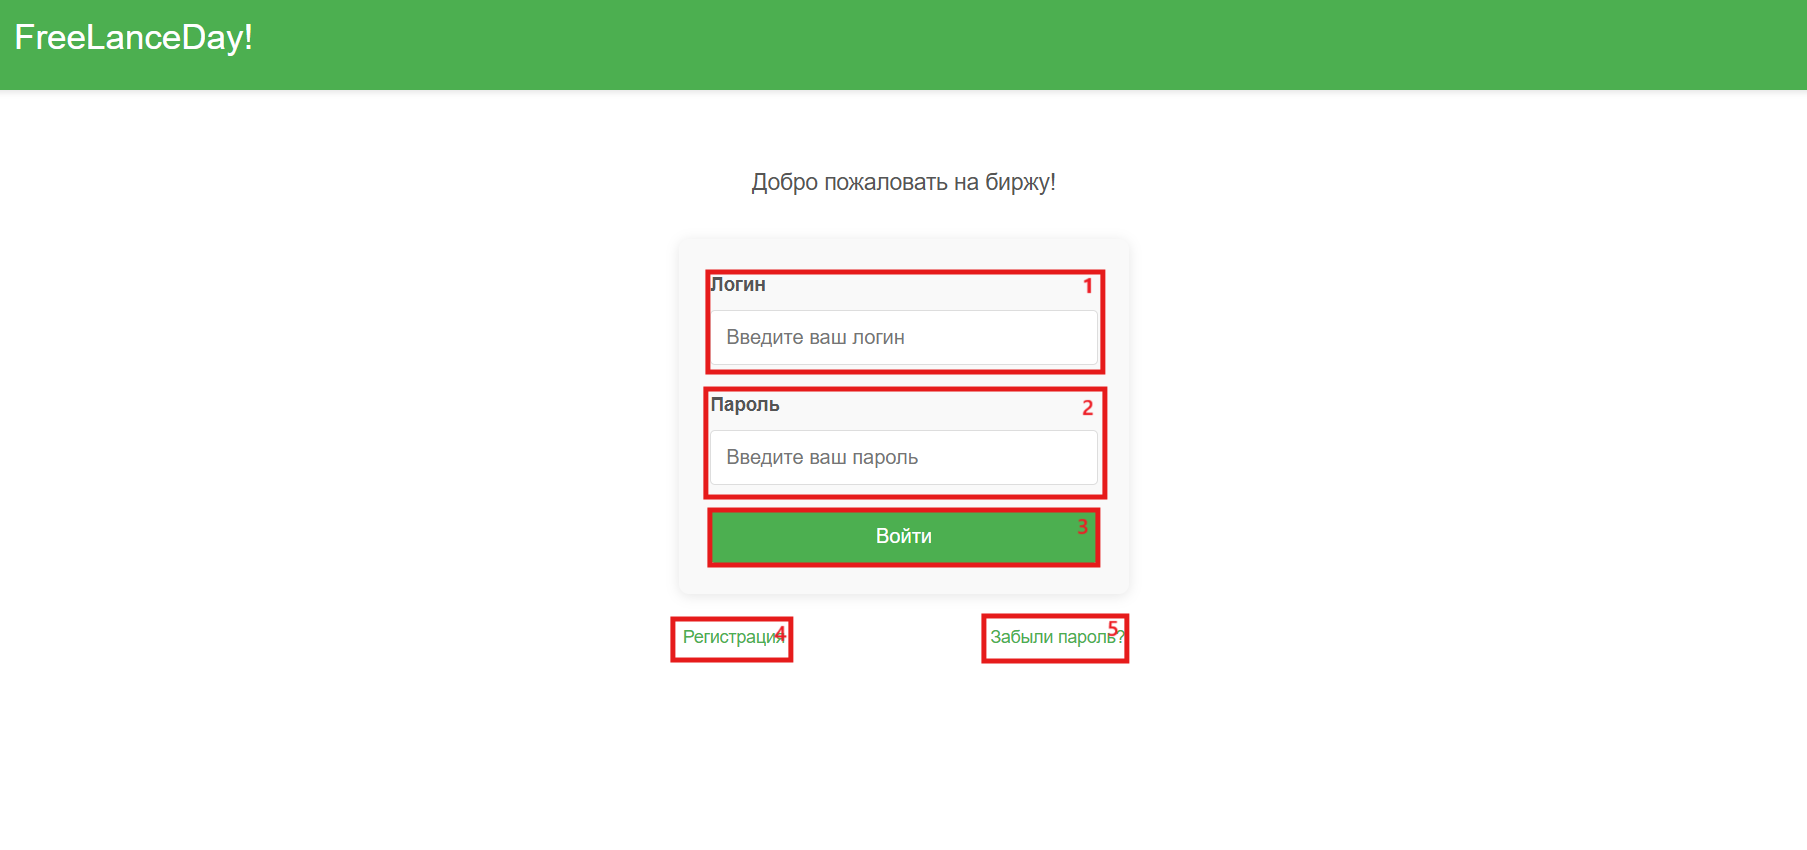
\includegraphics[width=1\linewidth]{maket1.png}}
	\caption{Макет страницы "<Страница входа">}
	\label{m1:image}
\end{figure}

На рисунке \ref{m2:image} представлен макет интерфейса страницы "<Создание задачи">. Макет содержит следующие элементы:

\begin{enumerate}
	\item Кнопка перехода в профиль авторизованного пользователя.
	\item Кнопка перехода к задачам авторизованного пользователя.
	\item Кнопка перехода к просмотру баланса авторизованного пользователя.
	\item Логин авторизованного пользователя.
	\item Кнопка выхода из аккаунта.
	\item Поле для ввода названия задачи.
	\item Поле для ввода описания задачи.
	\item Поле для ввода стоимости задачи.
	\item Выпадающий список для выбора сложности задачи.
	\item Кнопка отмены создания задачи.
	\item Кнопка создания задачи (неактивна).
\end{enumerate}
\clearpage

\begin{figure}[ht]
	\center{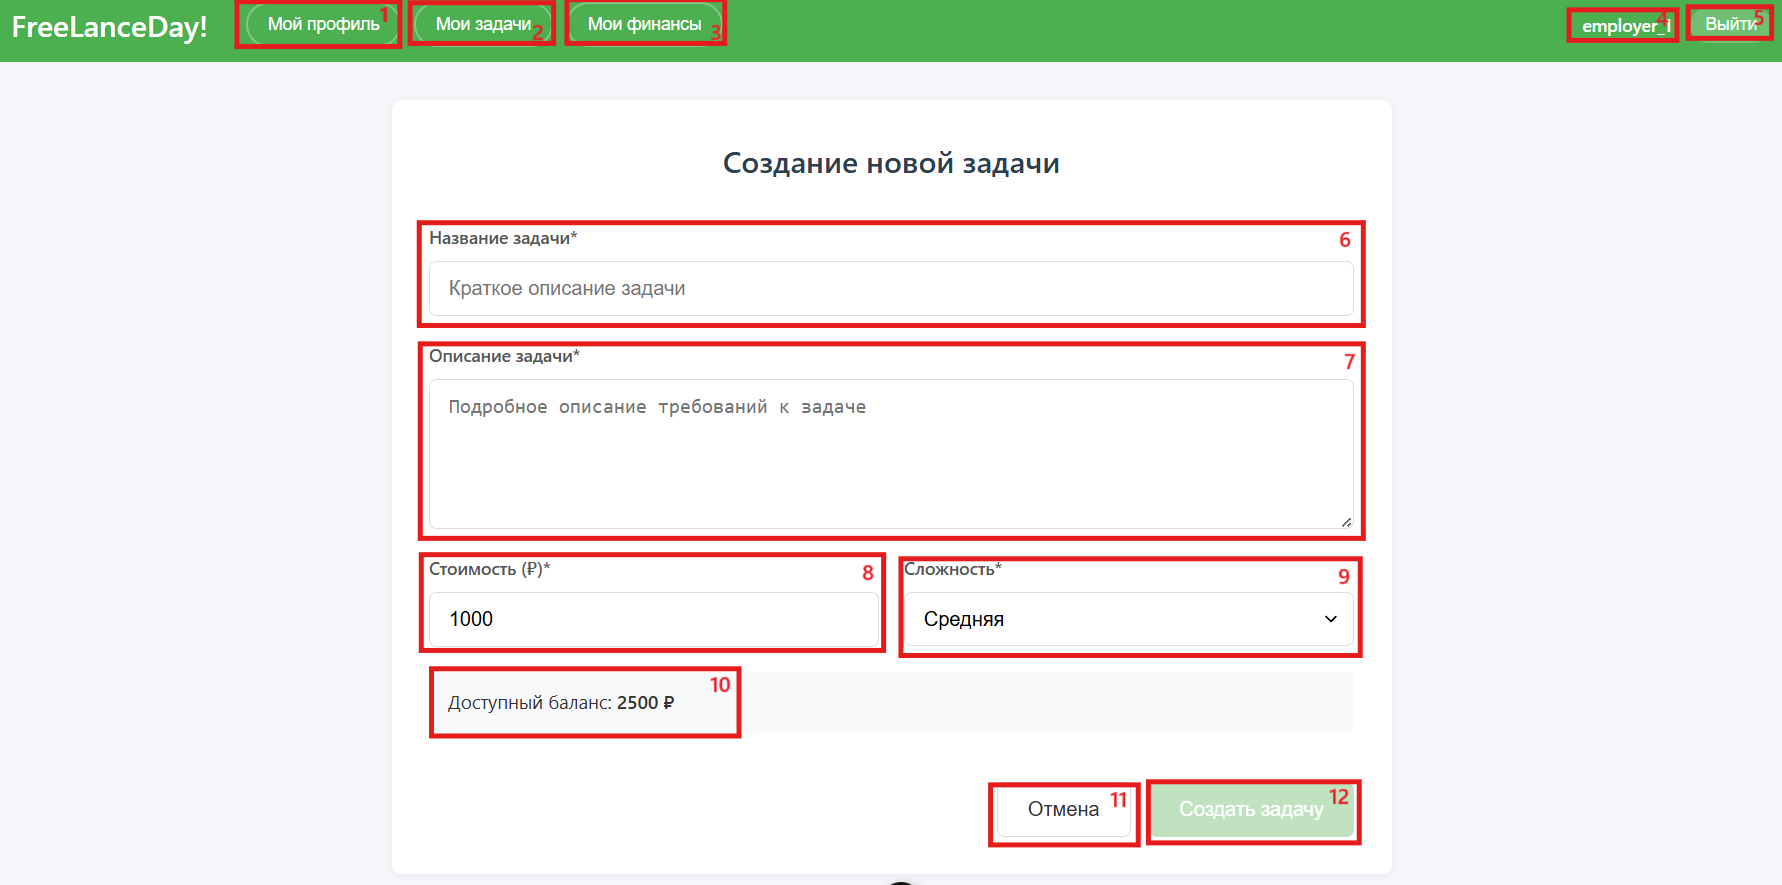
\includegraphics[width=1\linewidth]{maket2.png}}
	\caption{Макет страницы "<Создание задачи">}
	\label{m2:image}
\end{figure}

На рисунке \ref{m3:image} представлен макет интерфейса страницы "<Просмотр задач">. Макет содержит следующие элементы:

\begin{enumerate}
	\item Кнопка перехода в профиль авторизованного пользователя.
	\item Кнопка перехода к просмотру баланса авторизованного пользователя.
	\item Кнопка перехода к созданию задачи.
	\item Логин авторизованного пользователя.
	\item Кнопка выхода из аккаунта.
	\item Блок информации о задаче.
	\item Название задачи.
	\item Описание задачи.
	\item Стоимость задачи.
	\item Кнопка перехода к подробному описанию задачи.
\end{enumerate}
\clearpage

\begin{figure}[ht]
	\center{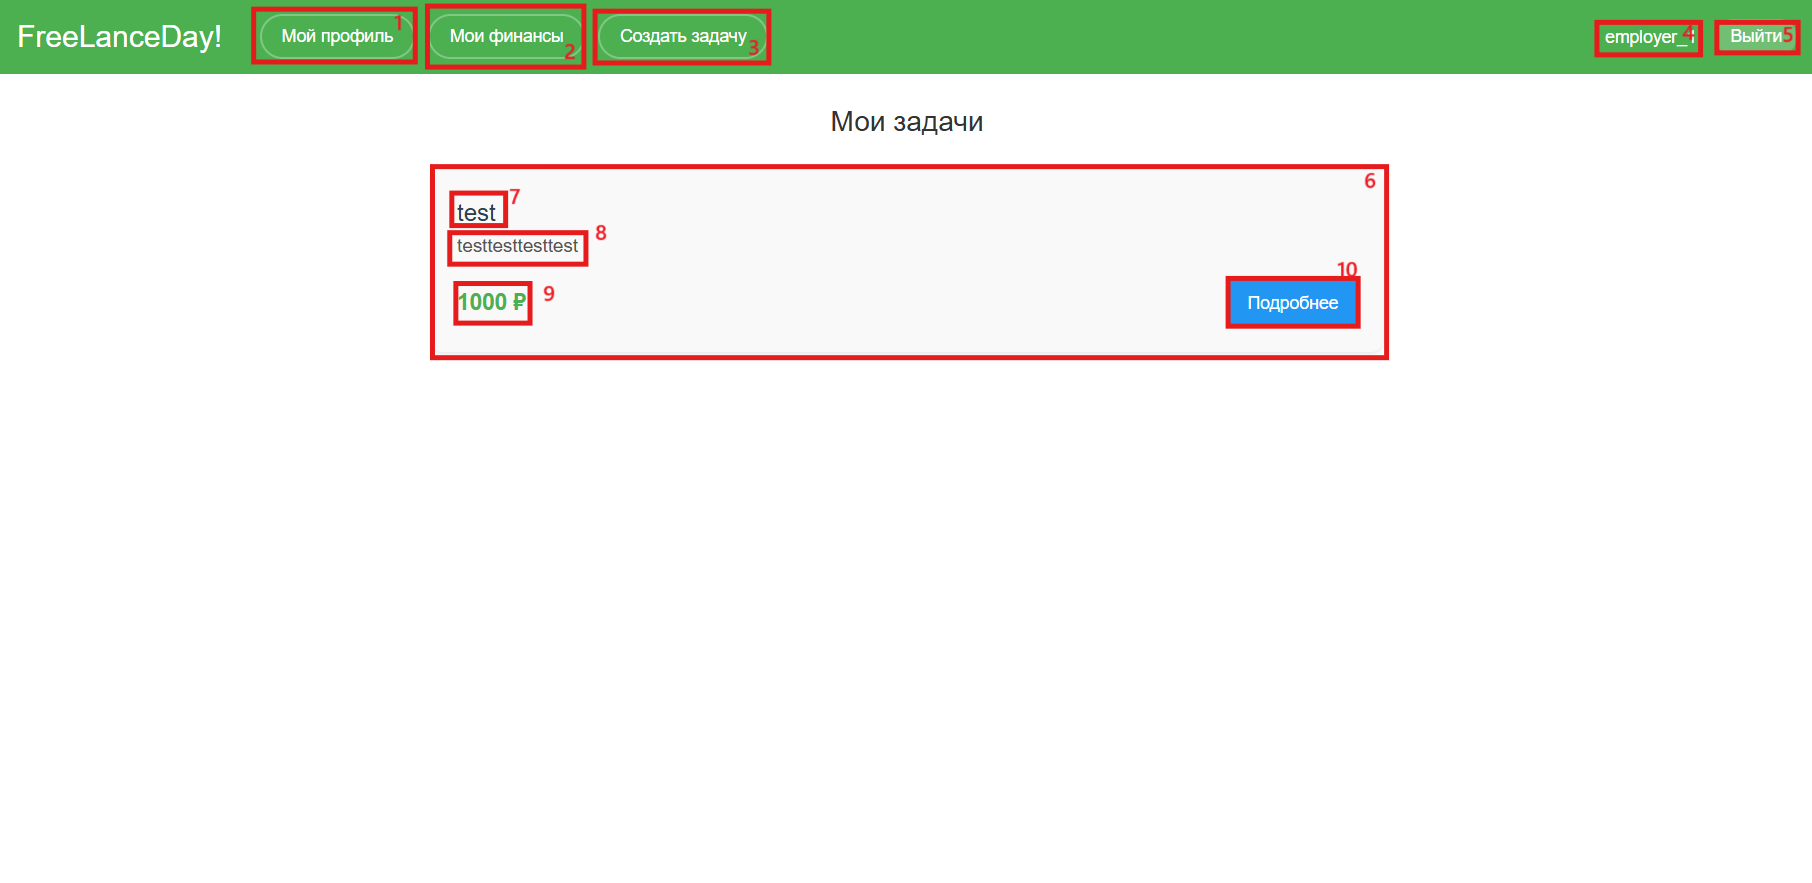
\includegraphics[width=1\linewidth]{maket3.png}}
	\caption{Макет страницы "<Просмотр задач">}
	\label{m3:image}
\end{figure}

На рисунке \ref{m4:image} представлен макет интерфейса страницы "<Просмотр баланса виртуального счёта">. Макет содержит следующие элементы:

\begin{enumerate}
	\item Кнопка перехода в профиль авторизованного пользователя.
	\item Кнопка перехода к задачам авторизованного пользователя.
	\item Кнопка перехода к созданию задачи.
	\item Логин авторизованного пользователя.
	\item Кнопка выхода из аккаунта.
	\item Баланс виртуального счёта авторизованного пользователя.
	\item Кнопка перехода к странице пополнения баланса.
	\item Блок истории операций.
	\item Блок информации о транзакции.
	\item Сумма транзакции.
	\item Тип транзакции.
	\item Описание транзакции.
	\item Дата транзакции.
\end{enumerate}
\clearpage

\begin{figure}[ht]
	\center{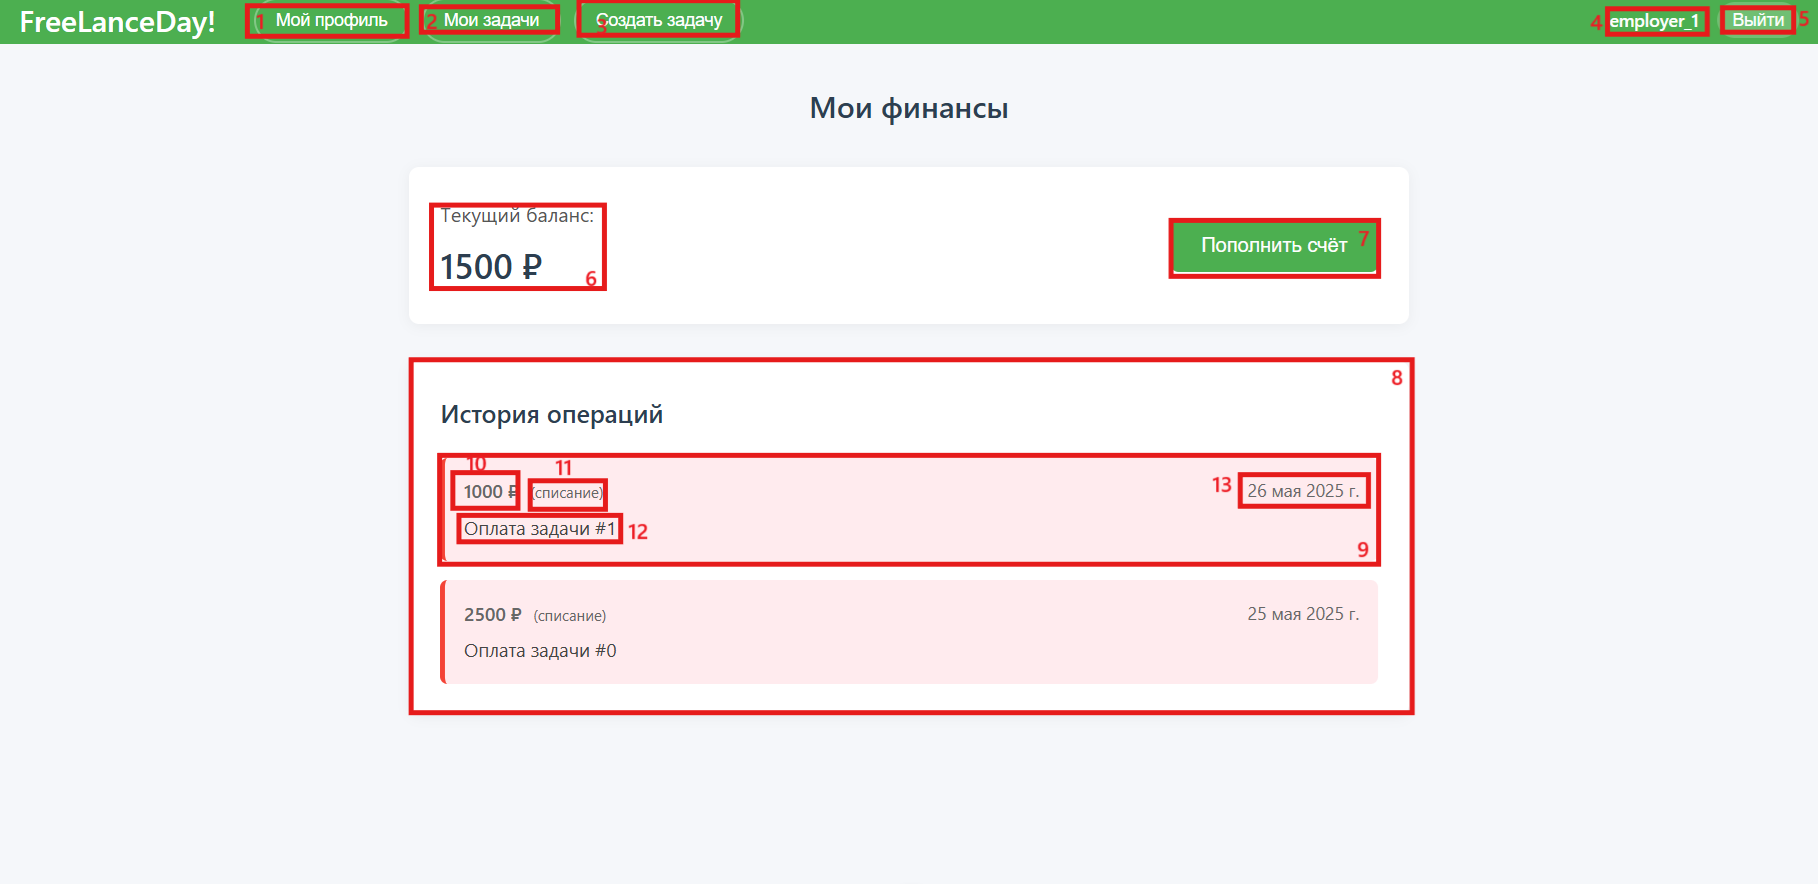
\includegraphics[width=1\linewidth]{maket4.png}}
	\caption{Макет страницы "<Просмотр баланса виртуального счёта">}
	\label{m4:image}
\end{figure}

На рисунке \ref{m5:image} представлен макет интерфейса страницы "<Просмотр профиля авторизованного пользователя">. Макет содержит следующие элементы:

\begin{enumerate}
	\item Кнопка перехода к задачам авторизованного пользователя.
	\item Кнопка перехода к просмотру баланса авторизованного пользователя.
	\item Кнопка перехода к созданию задачи.
	\item Логин авторизованного пользователя.
	\item Кнопка выхода из аккаунта.
	\item Дата создания аккаунта.
	\item Блок основной информации о пользователе.
	\item Имя пользователя.
	\item Организация пользователя.
	\item Описание пользователя.
	\item Кнопка перехода к редактированию профиля.
\end{enumerate}
\clearpage

\begin{figure}[ht]
	\center{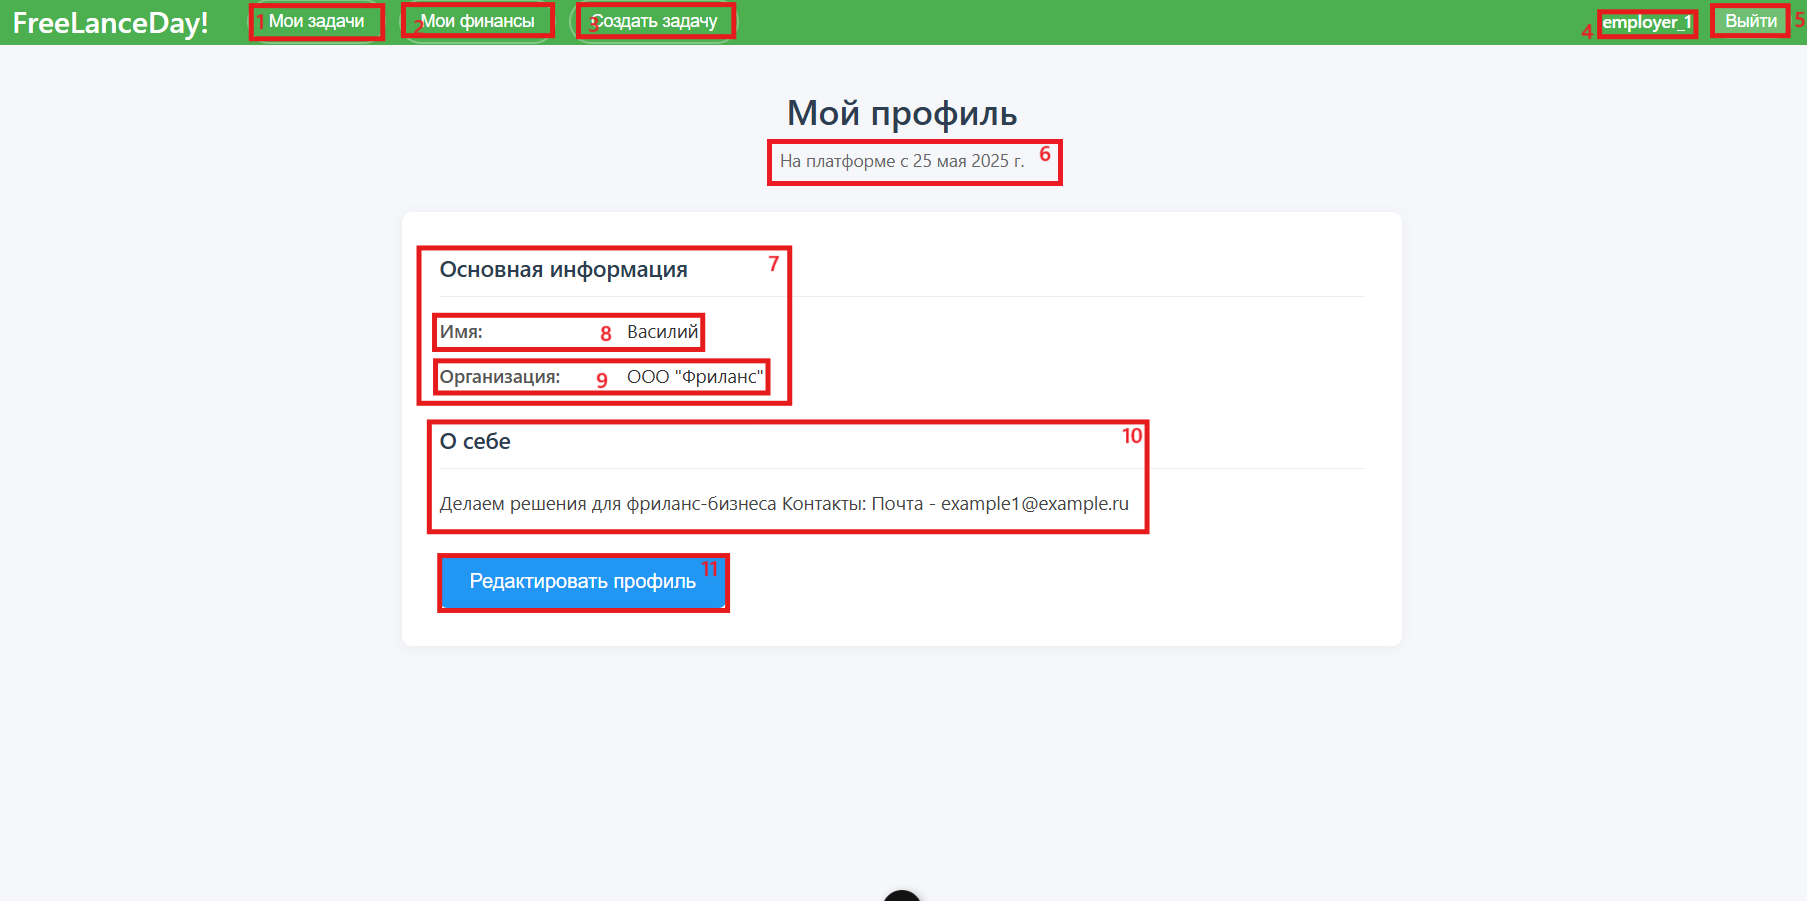
\includegraphics[width=1\linewidth]{maket5.png}}
	\caption{Макет страницы "<Просмотр профиля авторизованного пользователя">}
	\label{m5:image}
\end{figure}

На рисунке \ref{m6:image} представлен макет интерфейса страницы "<Пополнение виртуального счёта">. Макет содержит следующие элементы:

\begin{enumerate}
	\item Поле ввода суммы пополнения.
	\item Кнопки быстрого ввода суммы пополнения.
	\item Кнопки выбора способа оплаты.
	\item Поле ввода номера карты.
	\item Поле ввода срока действия карты.
	\item Поле ввода CVV/CVC кода карты.
	\item Кнопка пополнения счёта (неактивна).
\end{enumerate}
\clearpage

\begin{figure}[ht]
	\center{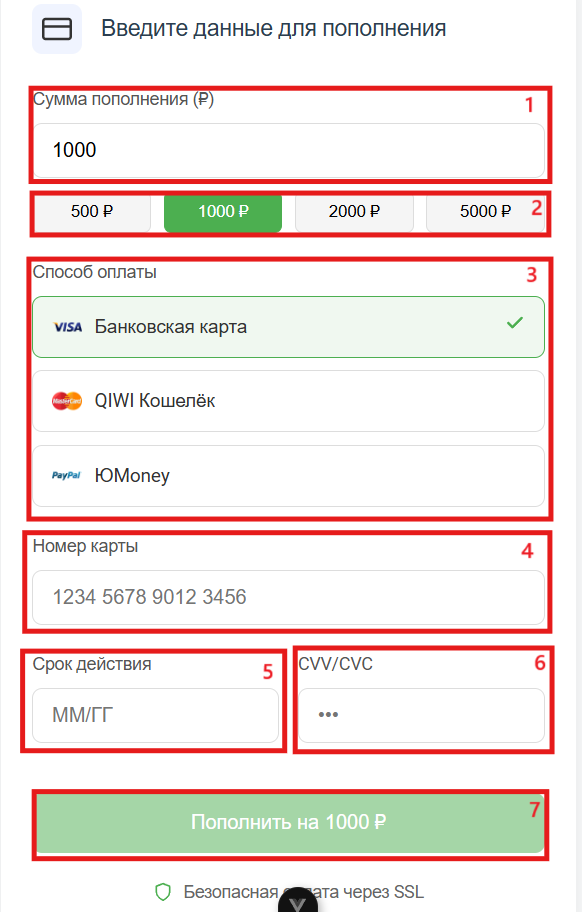
\includegraphics[width=0.7\linewidth]{maket6.png}}
	\caption{Макет страницы "<Пополнение виртуального счёта">}
	\label{m6:image}
\end{figure}

На рисунке \ref{m7:image} представлен макет интерфейса страницы "<Просмотр информации о задаче">. Макет содержит следующие элементы:

\begin{enumerate}
	\item Кнопка перехода в профиль авторизованного пользователя.
	\item Кнопка перехода к задачам авторизованного пользователя.
	\item Кнопка перехода к просмотру баланса авторизованного пользователя.
	\item Кнопка перехода к созданию задачи.
	\item Логин авторизованного пользователя.
	\item Кнопка выхода из аккаунта.
	\item Название задачи.
	\item Статус задачи.
	\item Стоимость задачи.
	\item Сложность задачи.
	\item Дата создания задачи.
	\item Заказчик, создавший задачу (ссылка на его профиль).
	\item Описание задачи.
	\item Кнопка перехода к просмотру откликов.
\end{enumerate}

\begin{figure}[ht]
	\center{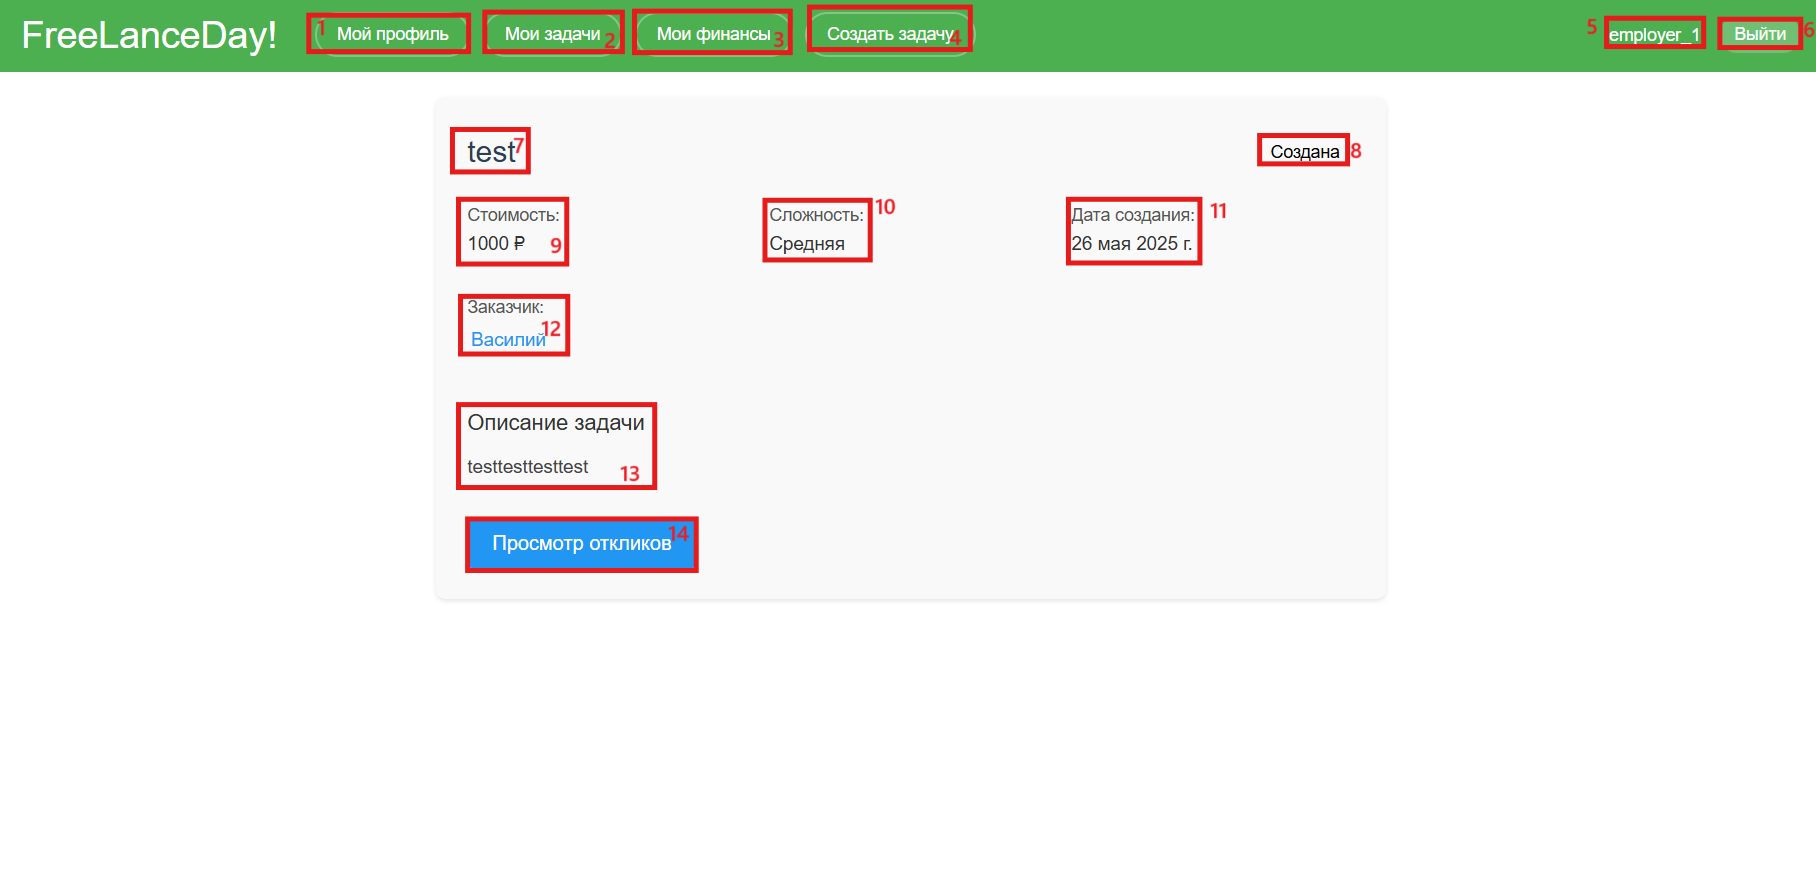
\includegraphics[width=1\linewidth]{maket7.png}}
	\caption{Макет страницы "<Просмотр информации о задаче">}
	\label{m7:image}
\end{figure}

На рисунке \ref{m8:image} представлен макет интерфейса страницы "<Просмотр откликов">. Макет содержит следующие элементы:

\begin{enumerate}
	\item Кнопка перехода в профиль авторизованного пользователя.
	\item Кнопка перехода к задачам авторизованного пользователя.
	\item Кнопка перехода к просмотру баланса авторизованного пользователя.
	\item Кнопка перехода к созданию задачи.
	\item Логин авторизованного пользователя.
	\item Кнопка выхода из аккаунта.
	\item Название страницы и название задачи, на котрую осуществляется просмотр откликов.
	\item Имя исполнителя (ссылка на его профиль).
	\item Уровень исполнителя.
	\item Уровень лояльности исполнителя.
	\item Кнопка назначения исполнителя на задачу.
	\item Дата регистрации исполнителя.
	\item Описание исполнителя.
\end{enumerate}

\begin{figure}[ht]
	\center{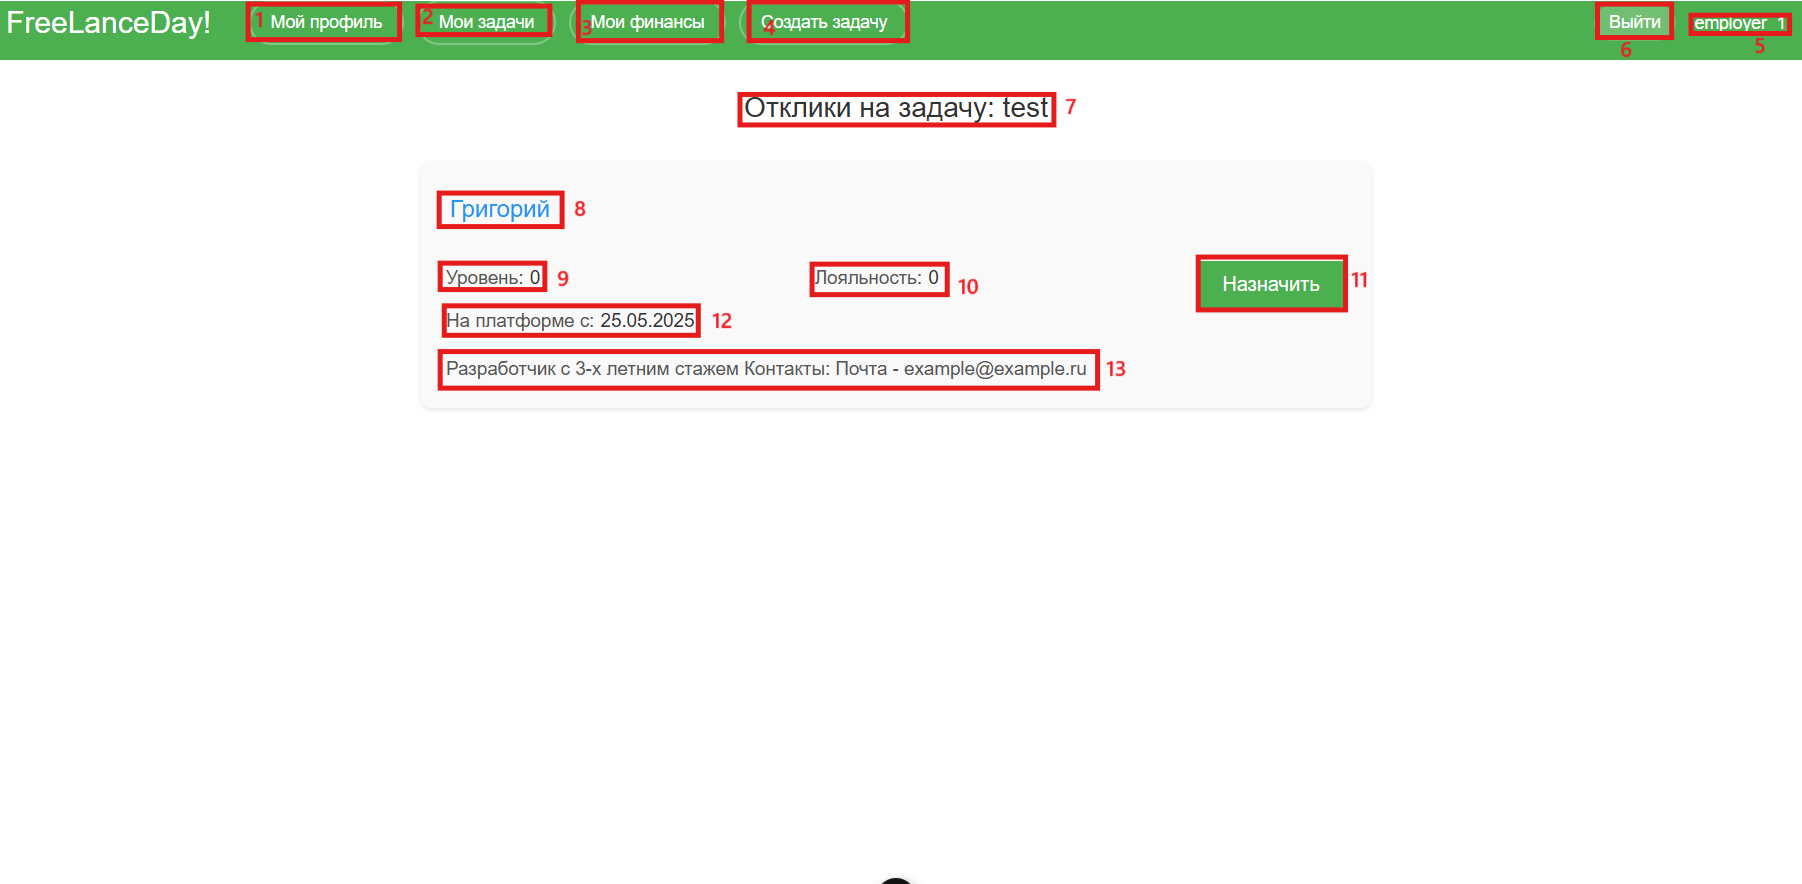
\includegraphics[width=1\linewidth]{maket8.png}}
	\caption{Макет страницы "<Просмотр откликов">}
	\label{m8:image}
\end{figure}
\ifПрактика{}\else{
   \section{Рабочий проект}
\subsection{Классы, используемые при разработке сайта}

Можно выделить следующий список классов и их методов, использованных при разработке web-приложения (таблица \ref{class:table}). Пример таблицы с уменьшенным межстрочным интервалом.

\renewcommand{\arraystretch}{0.8} % уменьшение расстояний до сетки таблицы
\begin{xltabular}{\textwidth}{|X|p{2.5cm}|>{\setlength{\baselineskip}{0.7\baselineskip}}p{4.85cm}|>{\setlength{\baselineskip}{0.7\baselineskip}}p{4.85cm}|}
\caption{Описание классов Bitrix, используемых в приложении\label{class:table}}\\
\hline \centrow \setlength{\baselineskip}{0.7\baselineskip} Название класса & \centrow \setlength{\baselineskip}{0.7\baselineskip} Модуль, к которому относится класс & \centrow Описание класса & \centrow Методы \\
\hline \centrow 1 & \centrow 2 & \centrow 3 & \centrow 4\\ \hline
\endfirsthead
\caption*{Продолжение таблицы \ref{class:table}}\\
\hline \centrow 1 & \centrow 2 & \centrow 3 & \centrow 4\\ \hline
\finishhead
CMain & Главный модуль & CMain – главный класс страницы web-приложения. После одного из этапов по загрузке страницы в сценарии становится доступным инициализированный системой объект данного класса с именем \$APPLICATION & void ShowTitle(string property\_code = «title», bool strip\_tags = true)
Выводит заголовок страницы
void SetTitle(string title)
Устанавливает заголовок страницы

void ShowCSS(bool external = true, bool XhtmlStyle = true)
Выводит таблицу стилей CSS страницы\\
\hline CFile & Главный модуль & CFile – Класс для работы с файлами и изображениями & array GetFileArray (int file\_id)
Метод возвращает массив, содержащий описание файла (путь к файлу, имя файла, размер) с идентификатором file\_id
\end{xltabular}
\renewcommand{\arraystretch}{1.0} % восстановление сетки

\subsection{Модульное тестирование разработанного web-сайта}

Модульный тест для класса User из модели данных представлен на рисунке \ref{unitUser:image}.

\begin{figure}[ht]
\begin{lstlisting}[language=Python]
from django.test import TestCase
from .models import *
User = get_user_model()


class ShpoTestCases(TestCase):

    def setUp(self) -> None:
        self.user = User.objects.create(username='testtestovich', password='testtestovich', first_name='Sad', last_name='')

    def test_2(self):

        self.assertEqual(self.user.first_name, 'Sad')
        self.assertEqual(self.user.last_name, 'Cat')
        print((self.user))
        print((self.user.first_name))
        print((self.user.last_name))
\end{lstlisting}  
\caption{Модульный тест класса User}
\label{unitUser:image}
\end{figure}

\subsection{Системное тестирование разработанного web-сайта}

На рисунке \ref{main:image} представлена главная страница сайта «Русатом – Аддитивные технологии».
\newpage % при необходимости можно переносить рисунок на новую страницу
\begin{figure}[H] % H - рисунок обязательно здесь, или переносится, оставляя пустоту
\center{\includegraphics[width=1\linewidth]{main1}}
\center{\includegraphics[width=1\linewidth]{main2}}
\center{\includegraphics[width=1\linewidth]{main3}}
\caption{Главная страница сайта «Русатом – Аддитивные технологии»}
\label{main:image}
\end{figure}

На рисунке \ref{menu:image} представлен динамический вывод заголовков, включающий в себя искомые фразы при поиске фраз.

\begin{figure}[ht]
\center{\includegraphics[width=1\linewidth]{menu}}
\caption{Динамический вывод заголовков}
\label{menu:image}
\end{figure}

На рисунке \ref{enter:image} представлен ввод данных для публикации новости.

\begin{figure}[ht]
\center{\includegraphics[width=1\linewidth]{enter}}
\caption{Ввод данных для публикации очень-очень длинной, интересной и полезной новости}
\label{enter:image}
\end{figure}

   \section*{ЗАКЛЮЧЕНИЕ}
\addcontentsline{toc}{section}{ЗАКЛЮЧЕНИЕ}

В ходе выполнения данной работы был разработан web сервис, реализующий функционал фриланс-биржи, опираясь на функционал уже существующих сервисов. Программная система реализована с использованием современных веб-технологий, включая Vue.js для клиентской части, Django для серверной части и СУБД PostgreSQL.

Основные результаты работы:

\begin{enumerate}
\item Проведен анализ предметной области. Рассмотрены принципы работы фриланс-биржи, выявлены положительные и отрицательные стороны конкурентов в данной сфере.
\item Разработана концептуальная модель web-сервиса. Разработана модель данных системы. Определены требования к системе.
\item Осуществлено проектирование web-сервиса. Разработана архитектура серверной части. Разработан пользовательский интерфейс web-сервиса.
\item Реализован и протестирован web-сервис. Проведено системное тестирование.
\end{enumerate}

Все требования, объявленные в техническом задании, были полностью реализованы, все задачи, поставленные в начале разработки проекта, были также решены.

Система готова к дальнейшему развитию, включая возможное добавление новых функций и улучшений.  

}\fi
\addcontentsline{toc}{section}{СПИСОК ИСПОЛЬЗОВАННЫХ ИСТОЧНИКОВ}

\begin{thebibliography}{9}
	
	\bibitem{javascript} Лутц, М. Изучаем Python / М. Лутц. – Москва: Символ-Плюс, 2022. – 1648 с. – ISBN 978-5-93286-159-5. – Текст: непосредственный.
	\bibitem{php} Бизли, Д. Python. Книга рецептов / Д. Бизли. – Москва: ДМК Пресс, 2020. – 464 с. – ISBN 978-5-97060-797-9. – Текст: непосредственный.
	\bibitem{css} Фельдман, В. Django 4. Практика создания веб-сайтов на Python / В. Фельдман. – Санкт-Петербург: БХВ-Петербург, 2023. – 512 с. – ISBN 978-5-9775-4061-2. – Текст: непосредственный.
	\bibitem{mysql}	Холи, У. Django для профессионалов / У. Холи. – Москва: Питер, 2021. – 448 с. – ISBN 978-5-4461-1451-8. – Текст: непосредственный.
	\bibitem{html5}	Клайн, К. PostgreSQL для начинающих / К. Клайн. – Москва: ДМК Пресс, 2019. – 368 с. – ISBN 978-5-97060-684-2. – Текст: непосредственный.
	\bibitem{htmlcss} Риггс, Г. PostgreSQL. Основы языка SQL / Г. Риггс. – Москва: Символ-Плюс, 2020. – 496 с. – ISBN 978-5-93286-231-8. – Текст: непосредственный.
	\bibitem{bigbook} Фримен, А. Практикум по программированию на JavaScript / А. Фримен. – Москва: Вильямс, 2013. – 960 с. – ISBN 978-5-8459-1799-7. – Текст: непосредственный.
	\bibitem{uchiru} Грегори, Н. Vue.js в действии / Н. Грегори. – Москва: ДМК Пресс, 2021. – 384 с. – ISBN 978-5-93700-123-0. – Текст: непосредственный.
	\bibitem{chaynik} Уильямс, Э. Vue.js. Полное руководство / Э. Уильямс. – Санкт-Петербург: Питер, 2023. – 528 с. – ISBN 978-5-4461-2345-9. – Текст: непосредственный.   
	\bibitem{22} Дакетт, Д. HTML и CSS. Разработка и дизайн веб-сайтов / Д. Дакетт. – Москва: Эксмо, 2022. – 480 с. – ISBN 978-5-04-160520-3. – Текст: непосредственный.   
	\bibitem{1231 Макфарланд, Д. Новая большая книга CSS / Д. Макфарланд. – Москва: Питер, 2021. – 720 с. – ISBN 978-5-4461-1452-5. – Текст: непосредственный.    
	\bibitem{servsssds} Чиннам, Р. Полный курс веб-разработки: Python, Django, JavaScript, Vue.js / Р. Чиннам. – Москва: Бомбора, 2023. – 896 с. – ISBN 978-5-04-170621-4. – Текст: непосредственный.
	\end{thebibliography}

\ifВКР{\appendix{Представление графического материала}

Графический материал, выполненный на отдельных листах,
изображен на рисунках А.1--А.\arabic{числоПлакатов}.
\setcounter{числоПлакатов}{0}

\renewcommand{\thefigure}{А.\arabic{figure}} % шаблон номера для плакатов

\begin{landscape}

\begin{плакат}
    
\includegraphics[width=0.82\linewidth]{Ramka1.eps}
    \заголовок{Сведения о ВКРБ}
    \label{pl1:image}      
\end{плакат}

\begin{плакат}
    
\includegraphics[width=0.82\linewidth]{Ramka2.eps}
    \заголовок{Цель и задачи разработки}
    \label{pl2:image}      
\end{плакат}

\begin{плакат}
    
\includegraphics[width=0.82\linewidth]{Ramka3.eps}
    \заголовок{Диаграмма прецендентов}
    \label{pl3:image}      
\end{плакат}

\begin{плакат}
    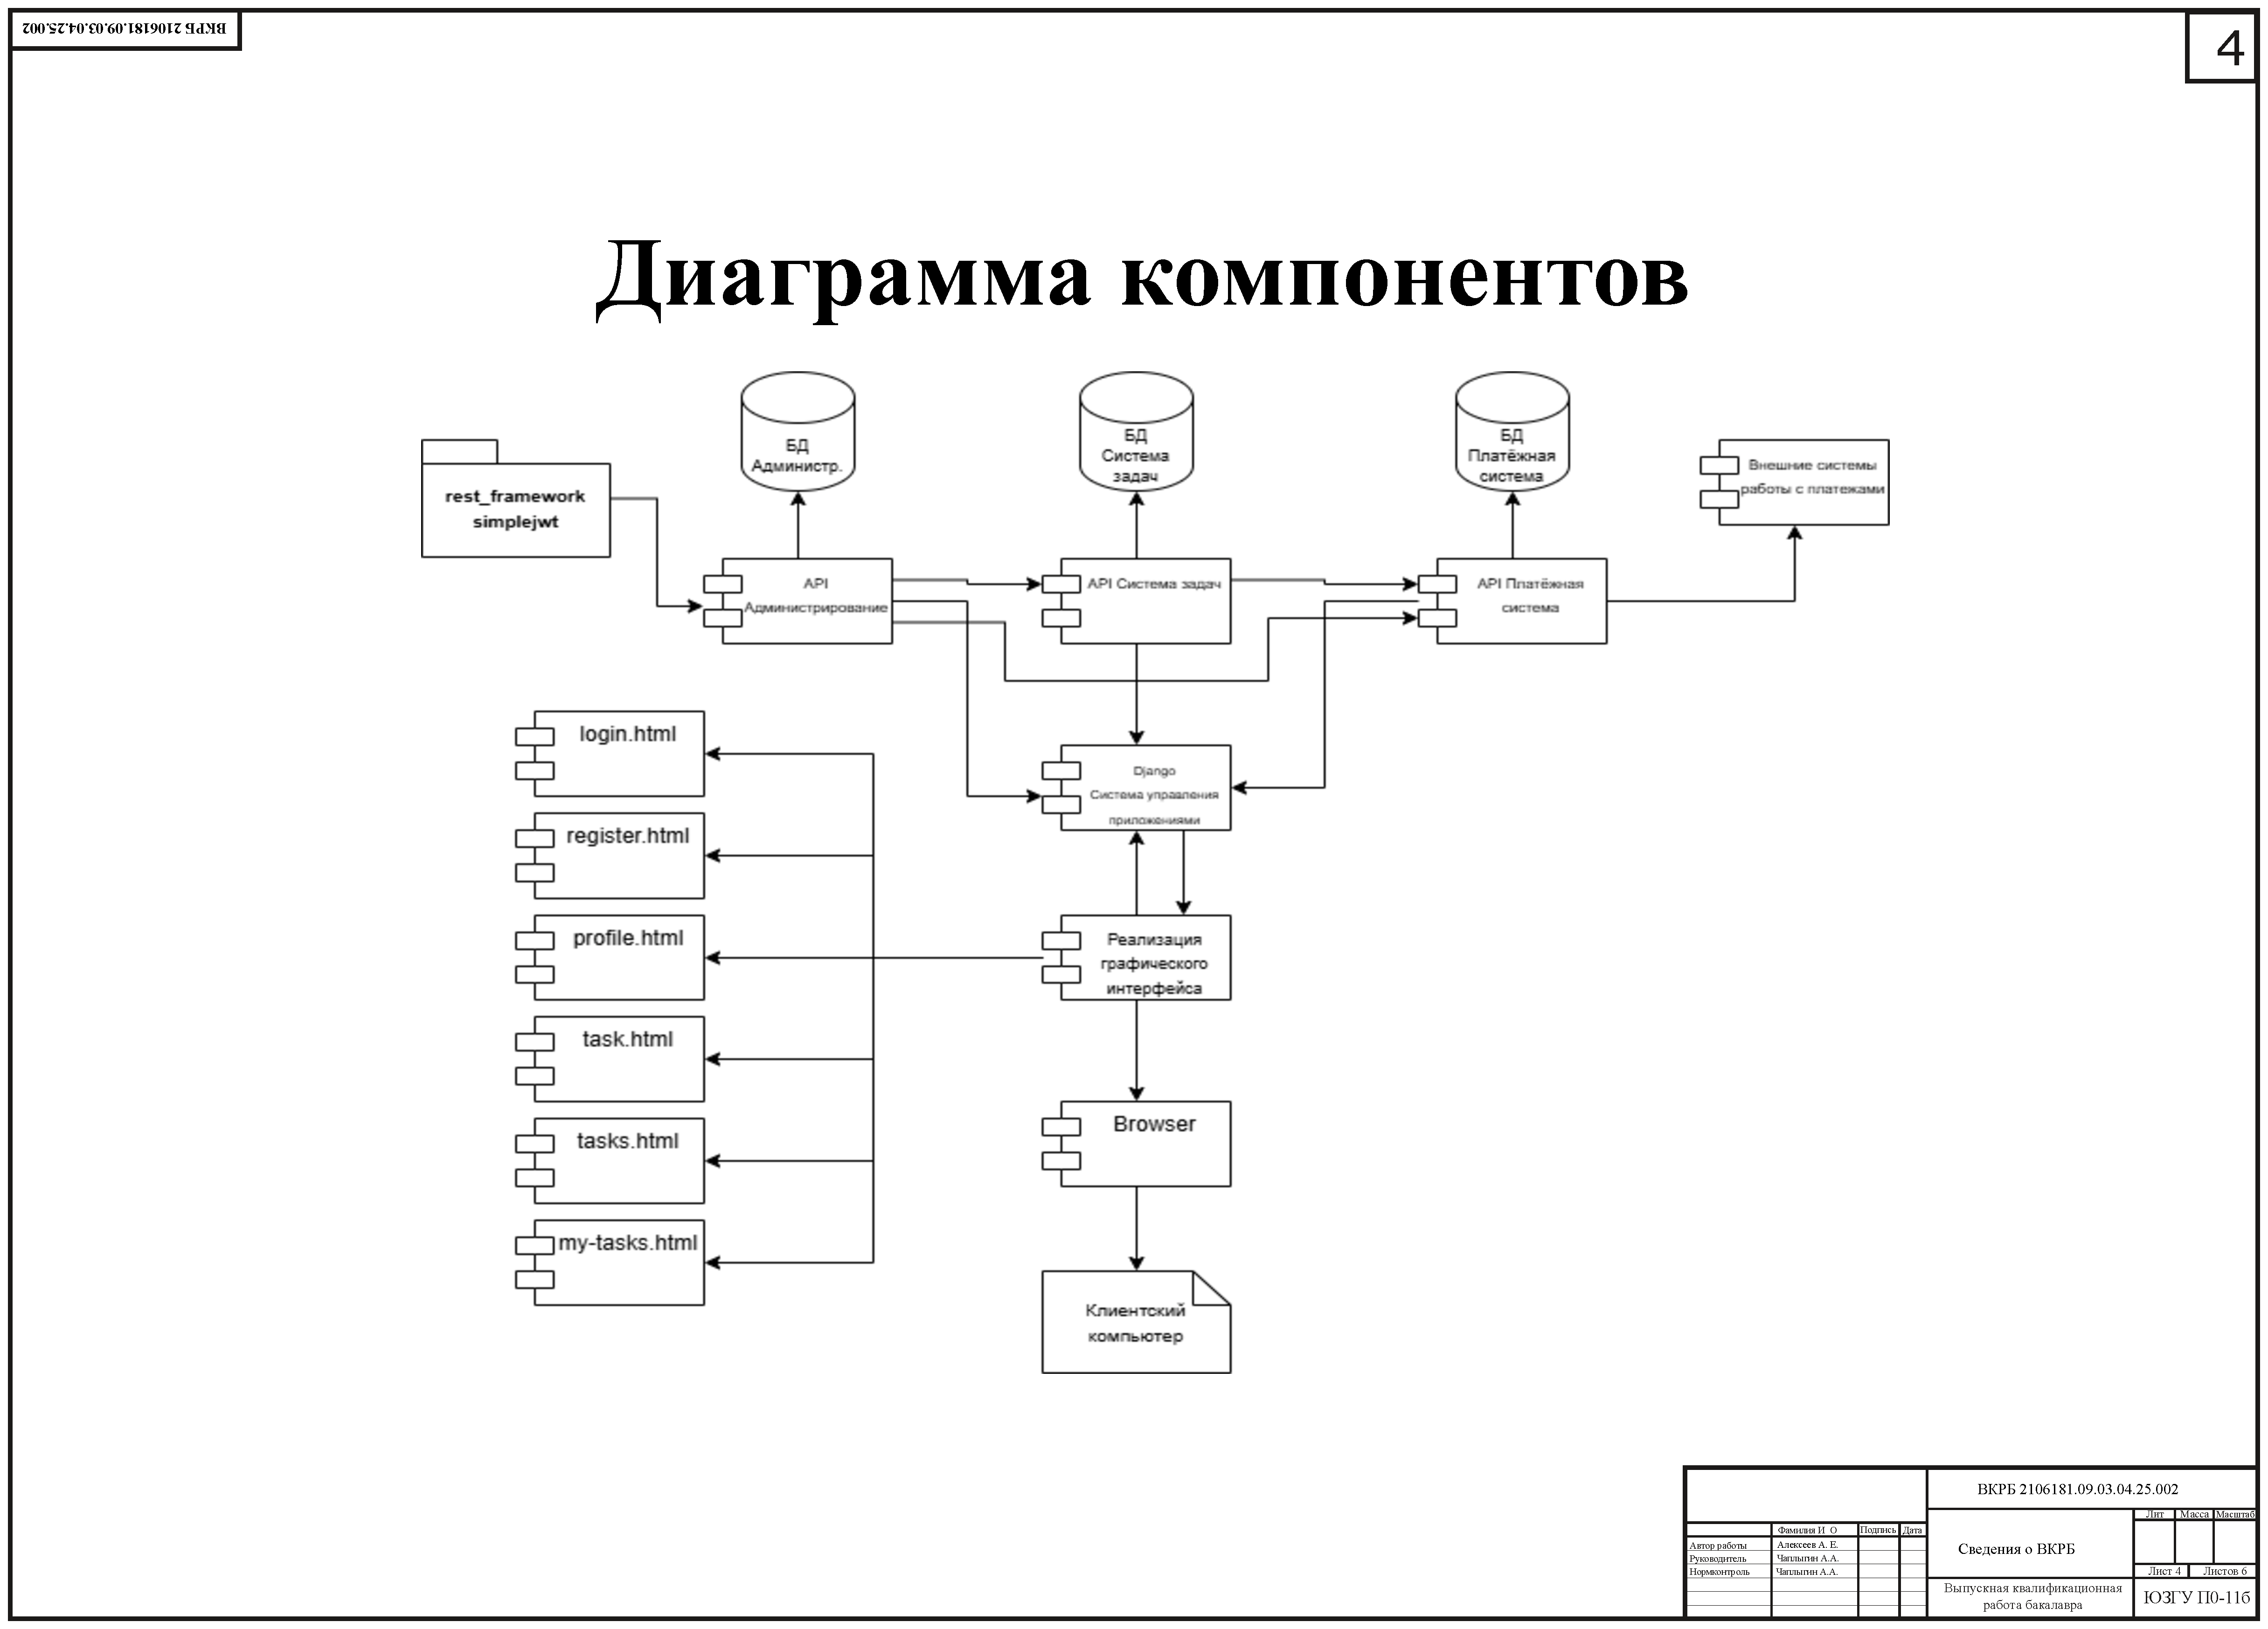
\includegraphics[width=0.82\linewidth]{Ramka4.eps}
    \заголовок{Диаграмма компонентов}
    \label{pl4:image}      
\end{плакат}

\begin{плакат}
	
\includegraphics[width=0.82\linewidth]{Ramka5.eps}
	\заголовок{Результат использования веб-сервиса}
	\label{pl5:image}      
\end{плакат}

\begin{плакат}
	
\includegraphics[width=0.82\linewidth]{Ramka6.eps}
	\заголовок{Заключение}
	\label{pl6:image}      
\end{плакат}

\end{landscape}
}\fi
\ifПрактика{}\else{\appendix{Фрагменты исходного кода программы}

viewsAdm.py
\lstinputlisting[language=Python, frame=none]{viewsAdm.py}

viewsTask.py
\lstinputlisting[language=Python, frame=none]{viewsTask.py}

viewsPay.py
\lstinputlisting[language=Python, frame=none]{viewsPay.py}

CreateTaskForm.vue
\lstinputlisting[language=HTML, frame=none]{CreateTaskForm.vue}

RegistrationForm.vue
\lstinputlisting[language=HTML, frame=none]{RegistrationForm.vue}

\ifВКР{
\newpage
\addcontentsline{toc}{section}{На отдельных листах (CD-RW в прикрепленном конверте)}
\noindent
\begin{tabular}{p{5.8cm}C{4.8cm}C{4.8cm}}
   Автор ВКР & \lhrulefill{\fill} & \fillcenter\Автор \\
            \setarstrut{\footnotesize}
           & \footnotesize{(подпись, дата)} & \\
            \restorearstrut
   Руководитель ВКР & \lhrulefill{\fill} & \fillcenter\Руководитель \\
            \setarstrut{\footnotesize}
           & \footnotesize{(подпись, дата)} & \\
            \restorearstrut
   Нормоконтроль & \lhrulefill{\fill} & \fillcenter\Нормоконтроль \\
            \setarstrut{\footnotesize}
           & \footnotesize{(подпись, дата)} & \\
            \restorearstrut
\end{tabular}
\vskip 2cm
\begin{center}
\textbf{Место для диска}
\end{center}
}\fi
}\fi
\end{document}
